\documentclass[11pt,a4paper]{article}
\usepackage{graphicx}
\usepackage{amssymb}
\usepackage{float}
\usepackage{amsmath}

\DeclareGraphicsExtensions{.pdf,.png,.jpg}

\begin{document}

\title{CS6690: Pattern Recognition Assignment \#3}
\author{Group 3: Akshay (ME10B124) \& Suthirth (ED10B059)}
\maketitle

\newpage

\section{Gaussian Mixture Models}
Gaussian Mixture Models are a type of classification that sets soft boundaries to data. It estimates data as a probabilistic mixture of its features. Each mixture is represented by by a gaussian density function in a gaussian mixture model.
$$
p(\bar{x}) = \sum\limits_{i=1}^K \pi_i N(\bar{x}|\mu_i, \Sigma_i)
$$
$K$ is the total number of classes, $\pi$ the weights. \\

Gaussian Mixture Models are solved using the Expectation maximization Algorithm (EM). This consists of calculating the posterior probability $\gamma$ which is calculated by using.

$$
\gamma_{nk} = \frac{\pi_k N(\bar{x}|\mu_k, \Sigma_k)}{\sum\limits_{i=1}^K \pi_i N(\bar{x}|\mu_i, \Sigma_i)}
$$
This posterior for each class gives us the contribution of class k to the mixture, using this, we can maximize the other parameters.
$$
\pi_k = \frac{\sum\limits_{i=1}^K \gamma_{nk}}{N}
$$ 
$$
\mu_k = \frac{1}{N_k} \sum\limits_{n=1}^N \gamma_{nk}\bar{x}_n
$$
$$
\Sigma_k = \frac{1}{N_k} \sum \limits_{n=1}^N \gamma_{nk}(\bar{x}_n - \mu_k)(\bar{x}_n - \mu_k)^T
$$
These three update equations are used to maximize and convergence is checked. The initial point for convergence is usually the k-means algorithm.
\newpage
\section{Dynamic Time Warping}
Dynamic Time Warping is a template matching algorithm that works by using the priciples of dynamic programming. It is a template matching that is capable of matching uneven templates as well. DTW aligns two sequence of feature vectors by warping the time axis iteratively until an optimal match between the two sequences is found. Using this, a distance measure can be computed, and can be used to match to a template.
\newline \\
Since we're dealing with continuous sequences in our dataset, the algorithm can be written as: \\ \\
D[i,j] = $|a[i] - b[j]|$ + min(D(i-1,j), D(i-1,j-1), D(i,j-1))
\section{Hidden Markov Models}
A Markov Model is one in which the current state of a system depends only on the present and previous states of the system. The order of the system tells us about the dependency of the nth previous value on the conditional probability density of the model. \\ \\

In a Hidden Markov Model, the state sequence is hidden as is the transition probabilities. We use the HMMs to characterize images and speech data. The performance of the HMM is also benchmarked to that of a GMM.

\section{Metrics}
The metrics used to evaluate the performance of a classifier are as follows
\begin{enumerate}
\item Precision
\item Recall
\item ROC Curves
\end{enumerate}
\newpage
\section{Image dataset}
\subsection{Data Exploration}
\begin{figure}[H]
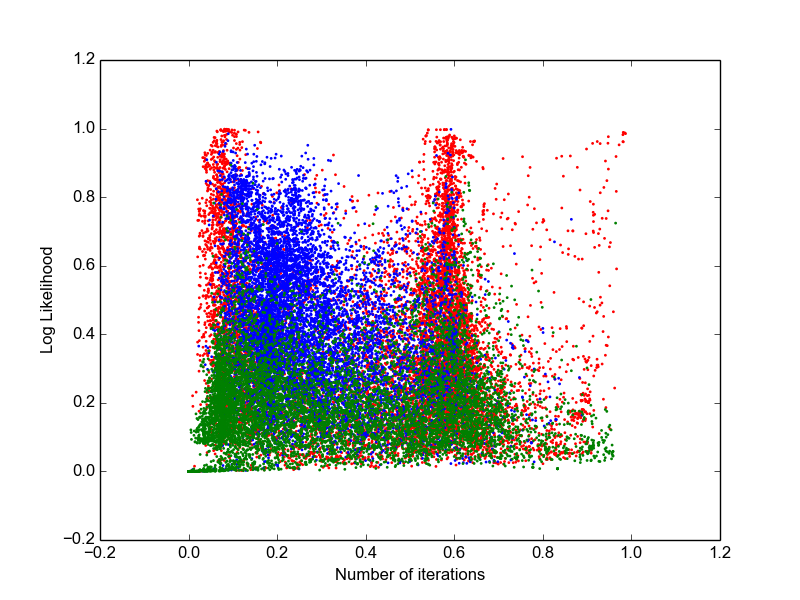
\includegraphics[width=.8\linewidth]{Figures/images_trainingdata_scatter.png}
\caption{Scatter plot of the image dataset}
\end{figure} 

Following images show mixture components for iterations 0, 5, 15 and 30.
\subsection{Coast}
Full Scatterplot: \\
\begin{minipage}[b]{0.25\textwidth}
\begin{figure}[H]
  \centering
  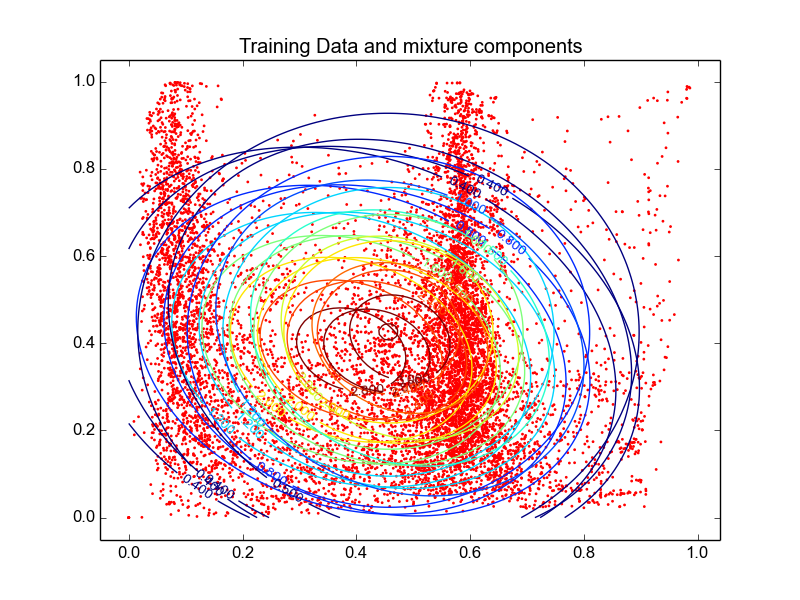
\includegraphics[width=.8\linewidth]{Figures/contourscoast0.png}
  \label{fig:sfig1}
\end{figure}%
\end{minipage}
\begin{minipage}[b]{0.25\textwidth}
\begin{figure}[H]
  \centering
  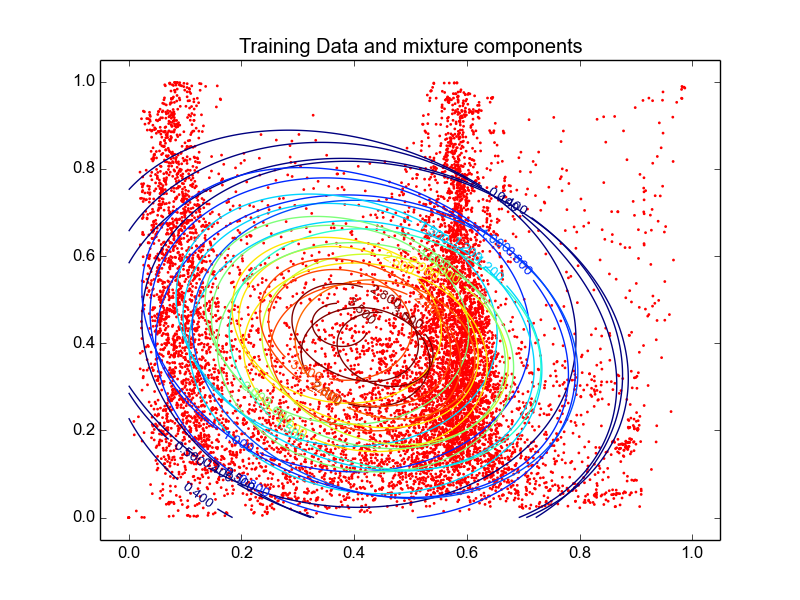
\includegraphics[width=.8\linewidth]{Figures/contourscoast5.png}

  \label{fig:sfig1}
\end{figure}%
\end{minipage}
\begin{minipage}[b]{0.25\textwidth}
\begin{figure}[H]
  \centering
  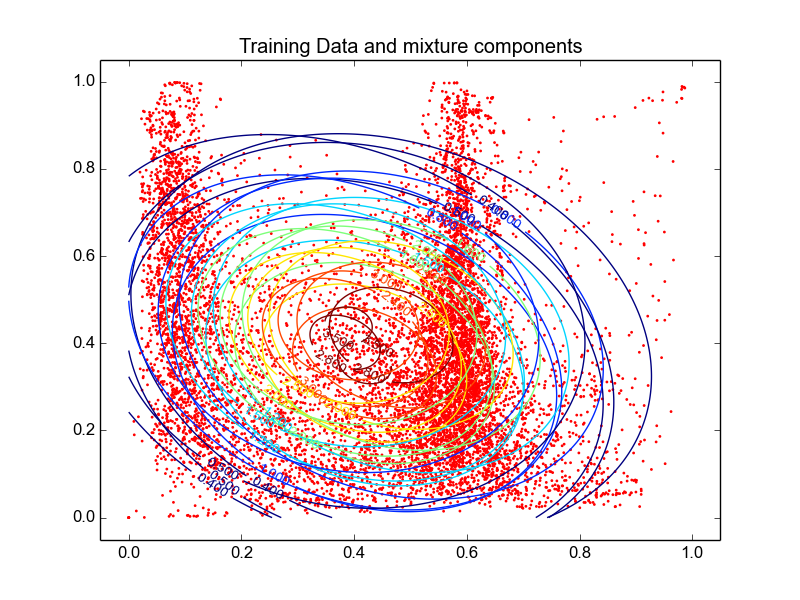
\includegraphics[width=.8\linewidth]{Figures/contourscoast15.png}

  \label{fig:sfig1}
\end{figure}%
\end{minipage}
\begin{minipage}[b]{0.25\textwidth}
\begin{figure}[H]
  \centering
  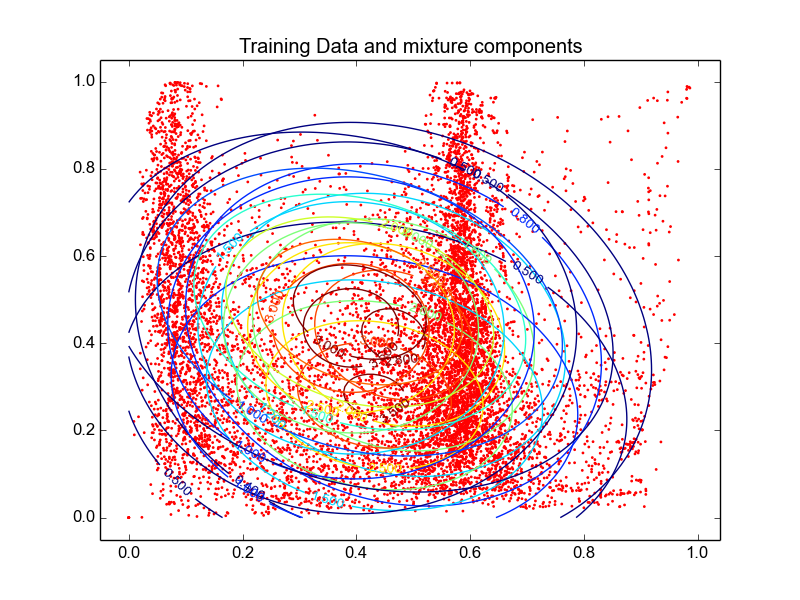
\includegraphics[width=.8\linewidth]{Figures/contourscoast30.png}

  \label{fig:sfig1}
\end{figure}%
\end{minipage}
\\
Diagonal Scatterplot: \\
\begin{minipage}[b]{0.25\textwidth}
\begin{figure}[H]
  \centering
  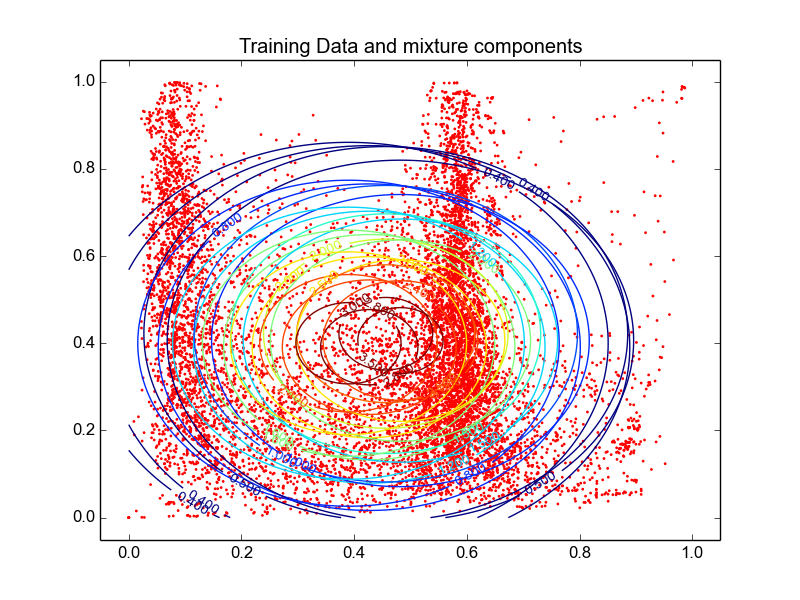
\includegraphics[width=.8\linewidth]{Figures/contours_diagcoast0.png}
\end{figure}%
\end{minipage}
\begin{minipage}[b]{0.25\textwidth}
\begin{figure}[H]
  \centering
  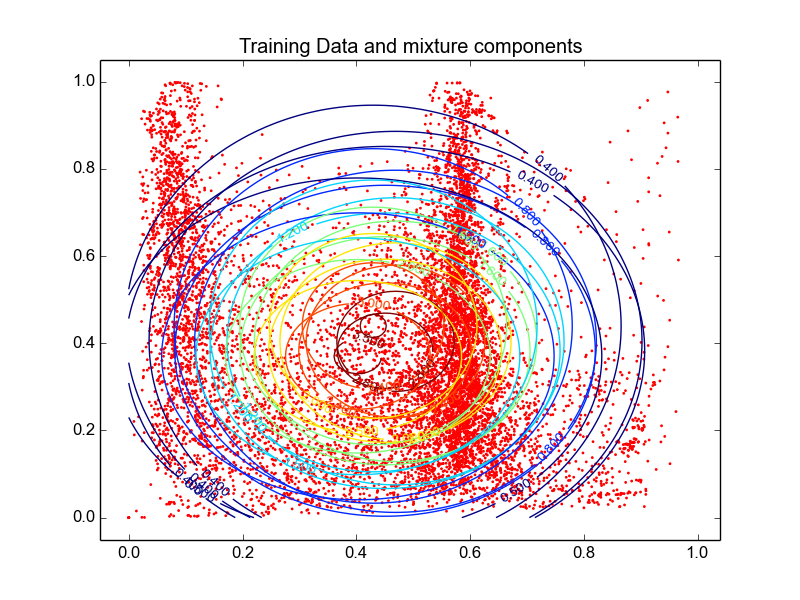
\includegraphics[width=.8\linewidth]{Figures/contours_diagcoast5.png}

  \label{fig:sfig1}
\end{figure}%
\end{minipage}
\begin{minipage}[b]{0.25\textwidth}
\begin{figure}[H]
  \centering
  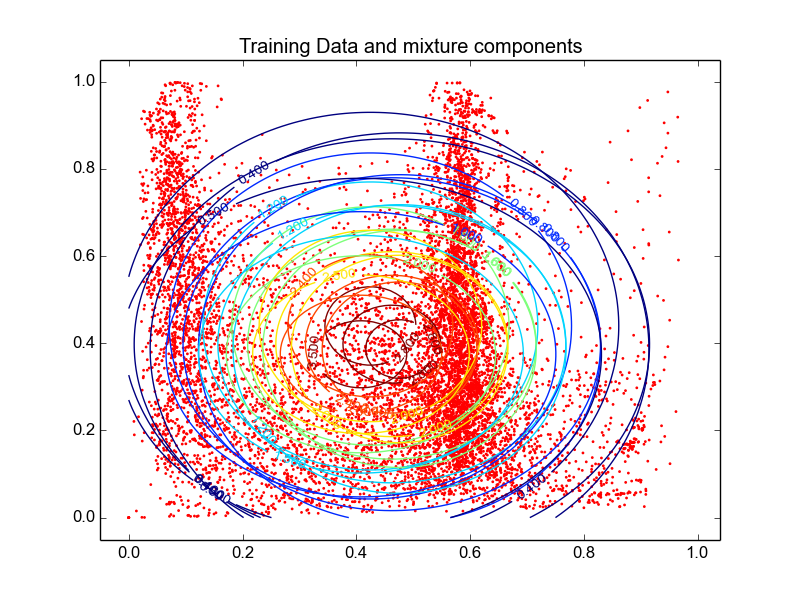
\includegraphics[width=.8\linewidth]{Figures/contours_diagcoast15.png}

  \label{fig:sfig1}
\end{figure}%
\end{minipage}
\begin{minipage}[b]{0.25\textwidth}
\begin{figure}[H]
  \centering
  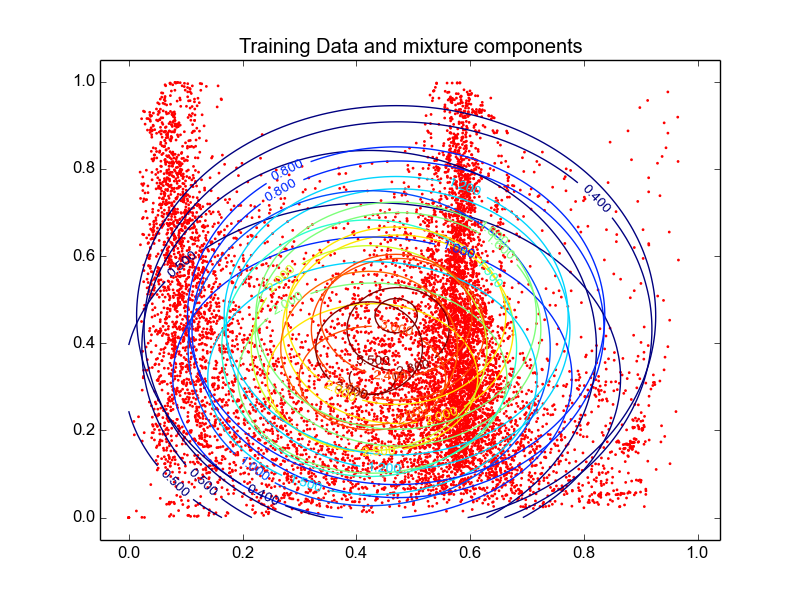
\includegraphics[width=.8\linewidth]{Figures/contours_diagcoast30.png}

  \label{fig:sfig1}
\end{figure}%
\end{minipage}
\subsection{Forest}
Full Scatterplot: \\
\begin{minipage}[b]{0.25\textwidth}
\begin{figure}[H]
  \centering
  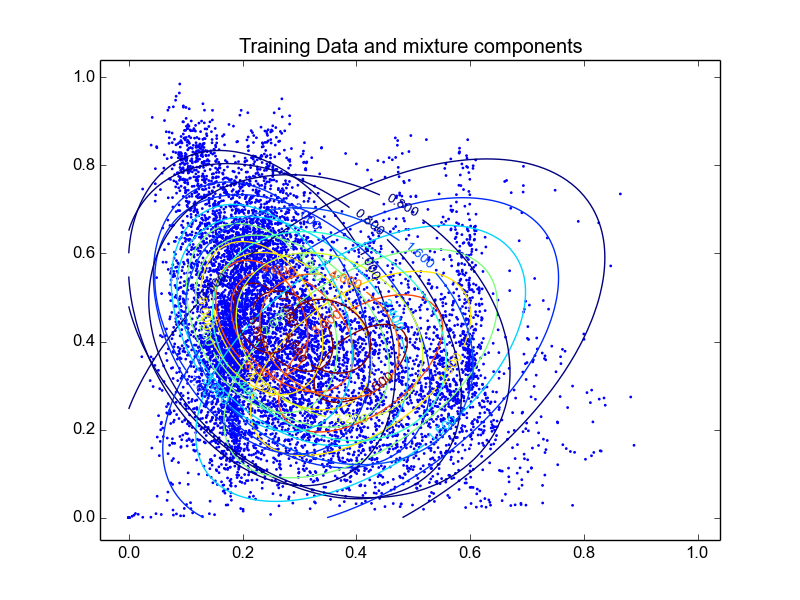
\includegraphics[width=.8\linewidth]{Figures/contoursforest0.png}
  \label{fig:sfig1}
\end{figure}%
\end{minipage}
\begin{minipage}[b]{0.25\textwidth}
\begin{figure}[H]
  \centering
  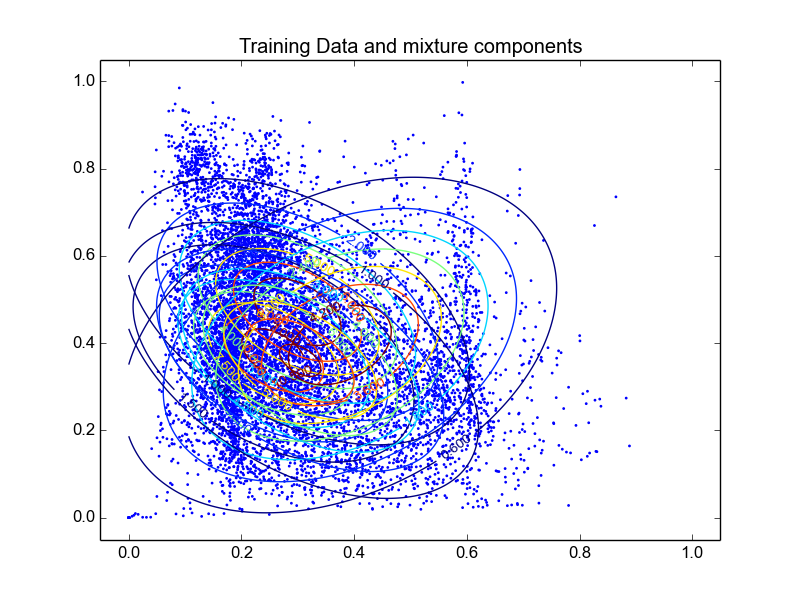
\includegraphics[width=.8\linewidth]{Figures/contoursforest5.png}

  \label{fig:sfig1}
\end{figure}%
\end{minipage}
\begin{minipage}[b]{0.25\textwidth}
\begin{figure}[H]
  \centering
  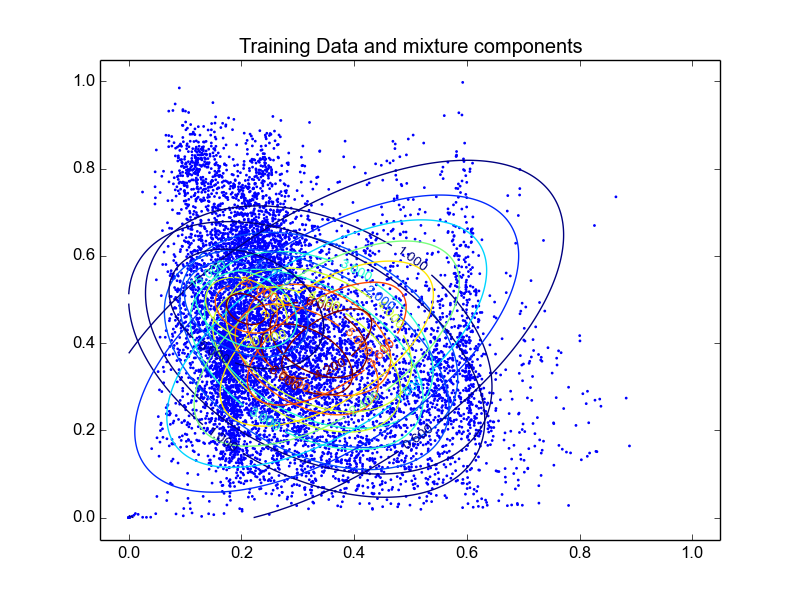
\includegraphics[width=.8\linewidth]{Figures/contoursforest15.png}

  \label{fig:sfig1}
\end{figure}%
\end{minipage}
\begin{minipage}[b]{0.25\textwidth}
\begin{figure}[H]
  \centering
  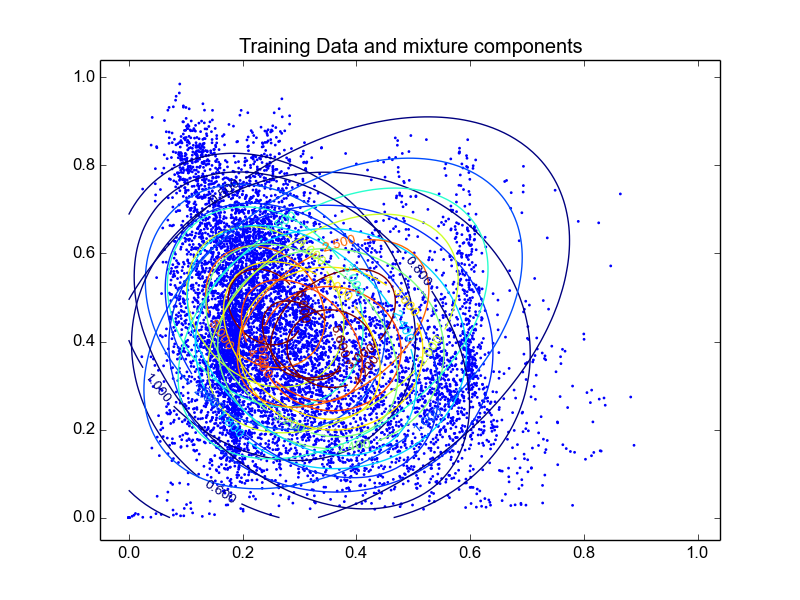
\includegraphics[width=.8\linewidth]{Figures/contoursforest30.png}

  \label{fig:sfig1}
\end{figure}%
\end{minipage}
\\
Diagonal Scatterplot: \\
\begin{minipage}[b]{0.25\textwidth}
\begin{figure}[H]
  \centering
  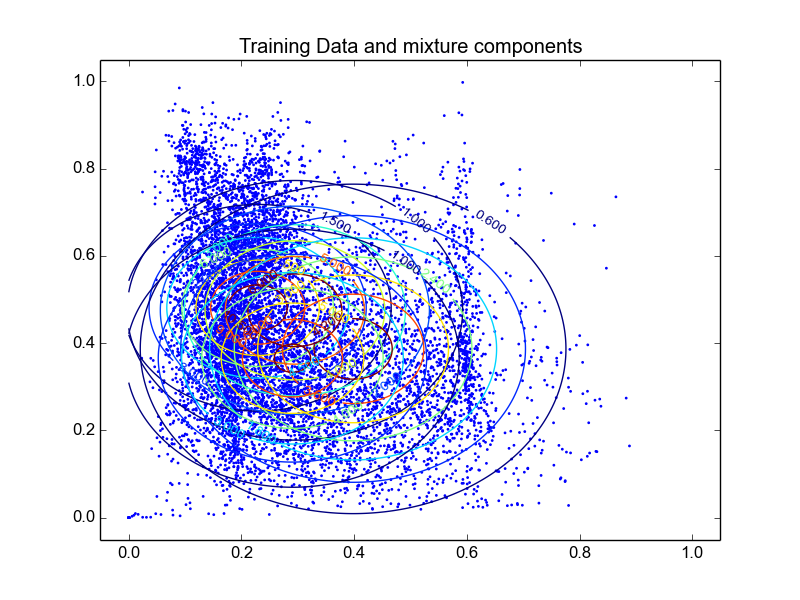
\includegraphics[width=.8\linewidth]{Figures/contours_diagforest0.png}
\end{figure}%
\end{minipage}
\begin{minipage}[b]{0.25\textwidth}
\begin{figure}[H]
  \centering
  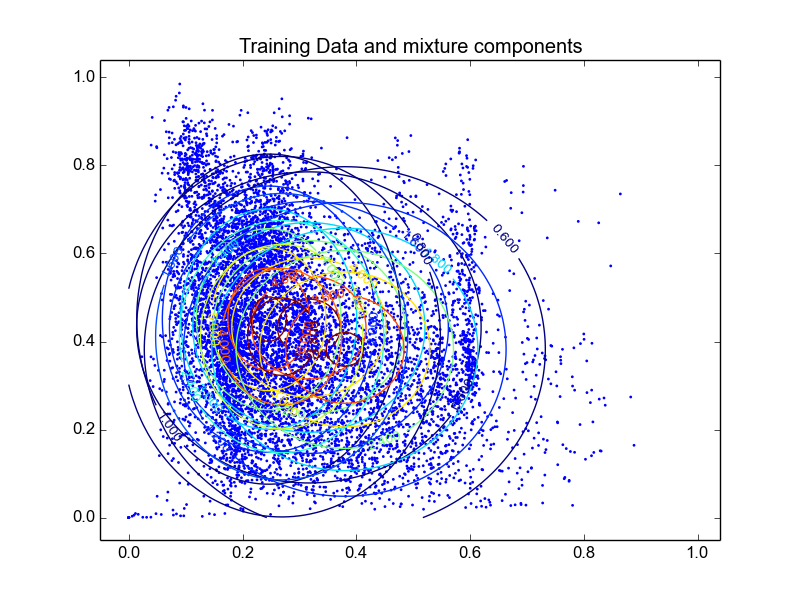
\includegraphics[width=.8\linewidth]{Figures/contours_diagforest5.png}

  \label{fig:sfig1}
\end{figure}%
\end{minipage}
\begin{minipage}[b]{0.25\textwidth}
\begin{figure}[H]
  \centering
  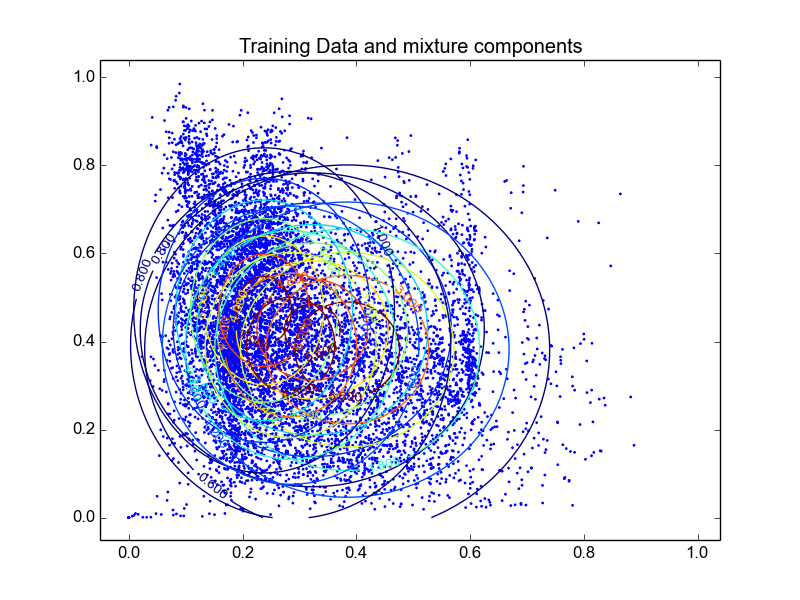
\includegraphics[width=.8\linewidth]{Figures/contours_diagforest15.png}

  \label{fig:sfig1}
\end{figure}%
\end{minipage}
\begin{minipage}[b]{0.25\textwidth}
\begin{figure}[H]
  \centering
  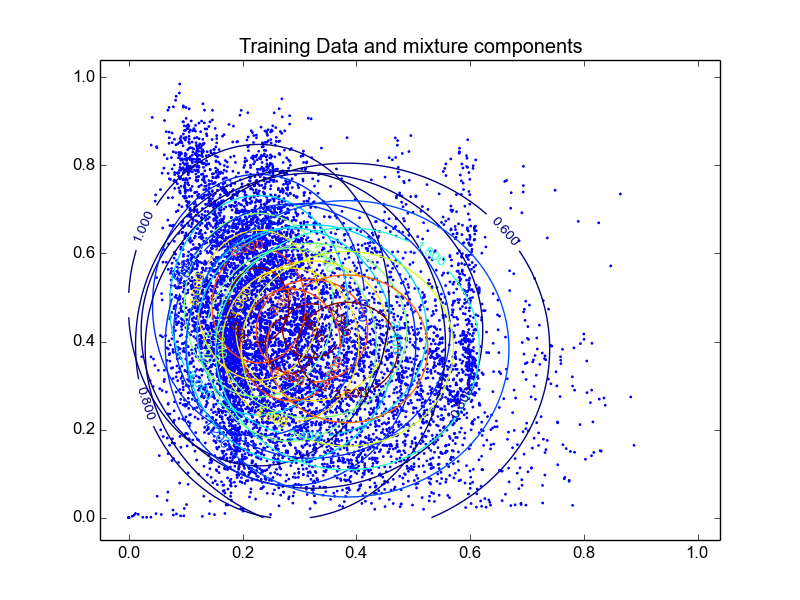
\includegraphics[width=.8\linewidth]{Figures/contours_diagforest30.png}

  \label{fig:sfig1}
\end{figure}%
\end{minipage}
\subsection{Street}
Full Scatterplot: \\
\begin{minipage}[b]{0.25\textwidth}
\begin{figure}[H]
  \centering
  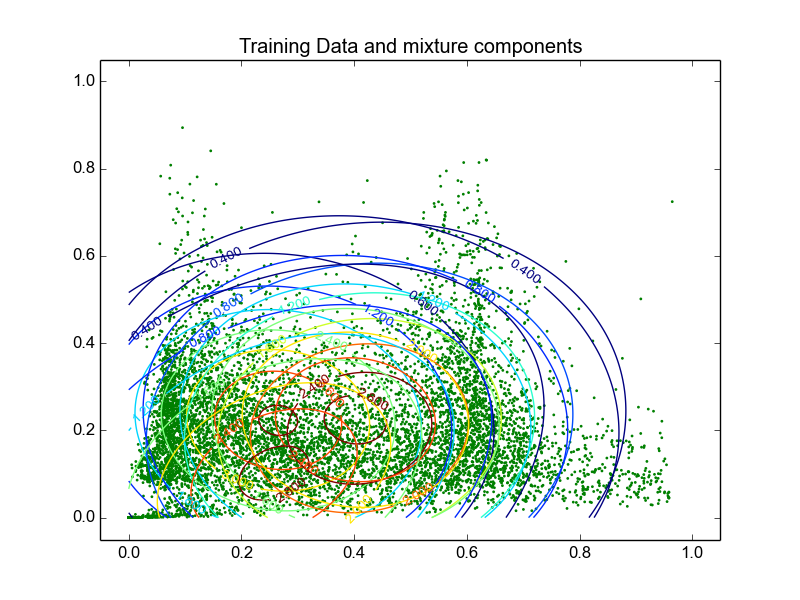
\includegraphics[width=.8\linewidth]{Figures/contoursstreet0.png}
  \label{fig:sfig1}
\end{figure}%
\end{minipage}
\begin{minipage}[b]{0.25\textwidth}
\begin{figure}[H]
  \centering
  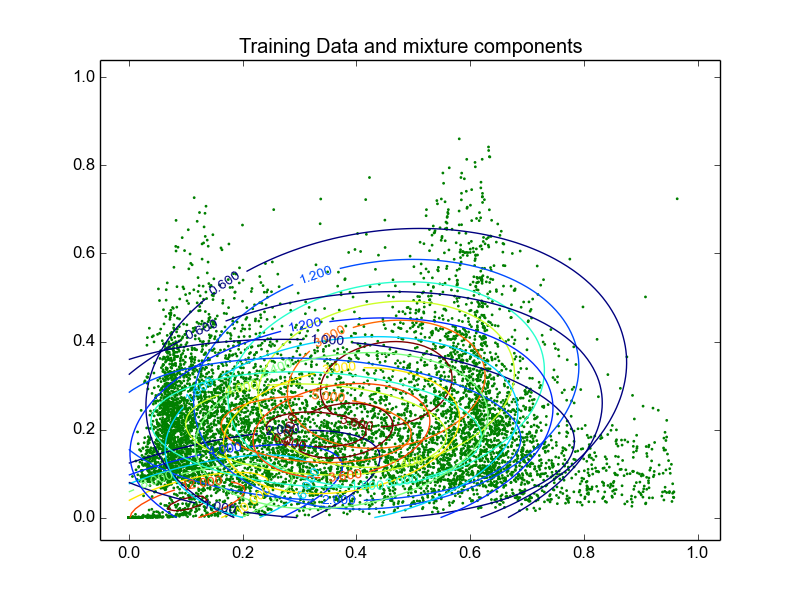
\includegraphics[width=.8\linewidth]{Figures/contoursstreet5.png}

  \label{fig:sfig1}
\end{figure}%
\end{minipage}
\begin{minipage}[b]{0.25\textwidth}
\begin{figure}[H]
  \centering
  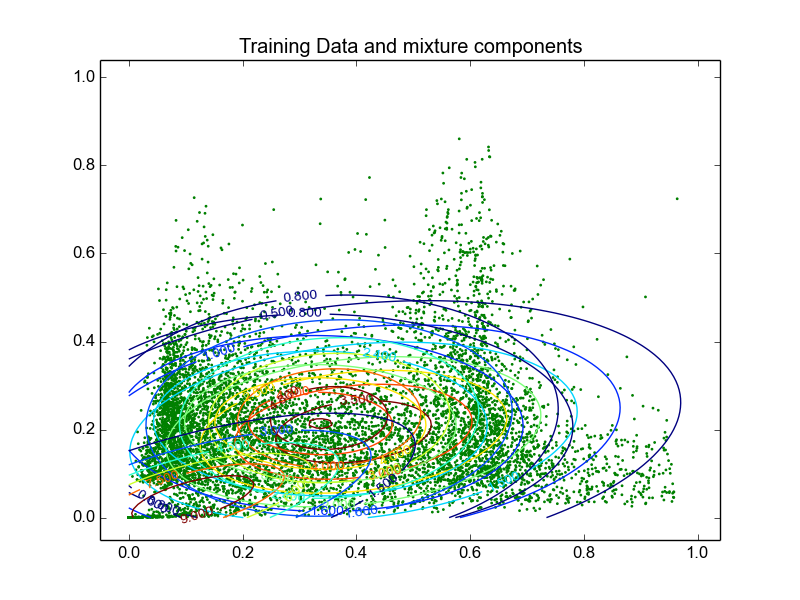
\includegraphics[width=.8\linewidth]{Figures/contoursstreet15.png}

  \label{fig:sfig1}
\end{figure}%
\end{minipage}
\begin{minipage}[b]{0.25\textwidth}
\begin{figure}[H]
  \centering
  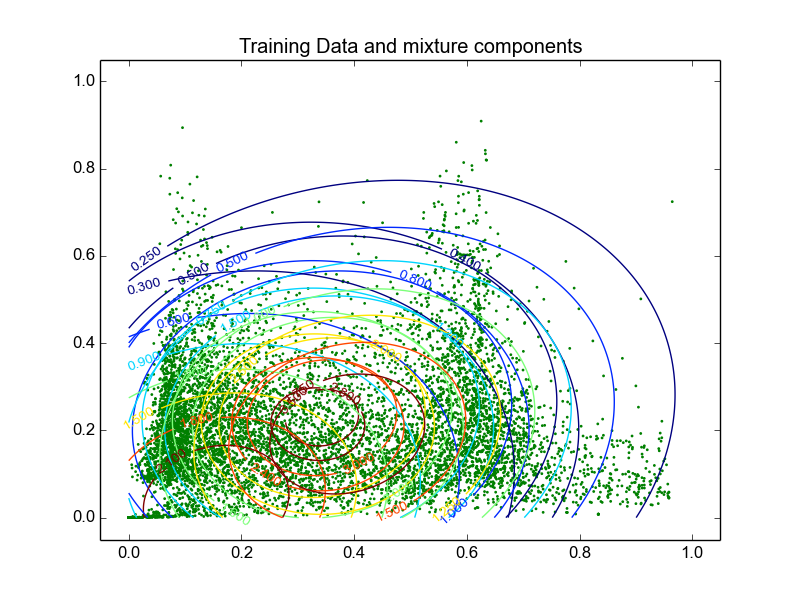
\includegraphics[width=.8\linewidth]{Figures/contoursstreet30.png}

  \label{fig:sfig1}
\end{figure}%
\end{minipage}
\\
Diagonal Scatterplot: \\
\begin{minipage}[b]{0.25\textwidth}
\begin{figure}[H]
  \centering
  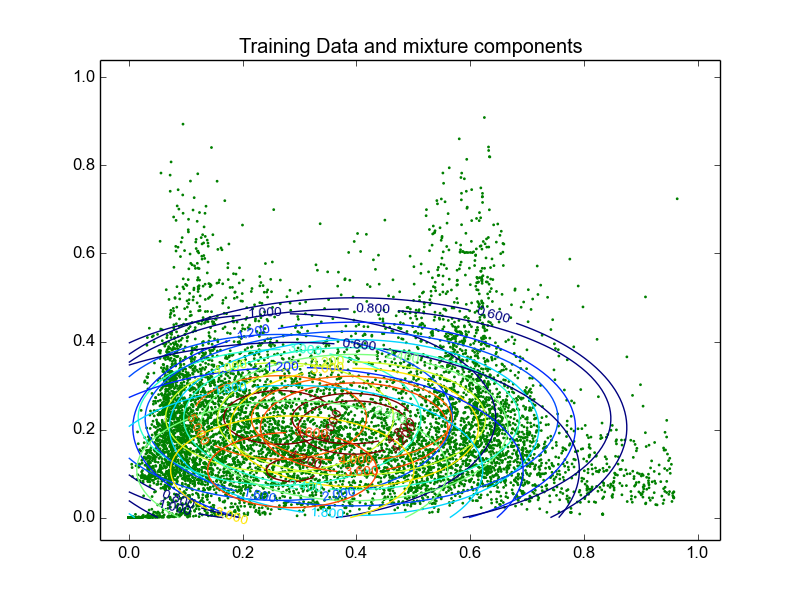
\includegraphics[width=.8\linewidth]{Figures/contours_diagstreet0.png}
\end{figure}%
\end{minipage}
\begin{minipage}[b]{0.25\textwidth}
\begin{figure}[H]
  \centering
  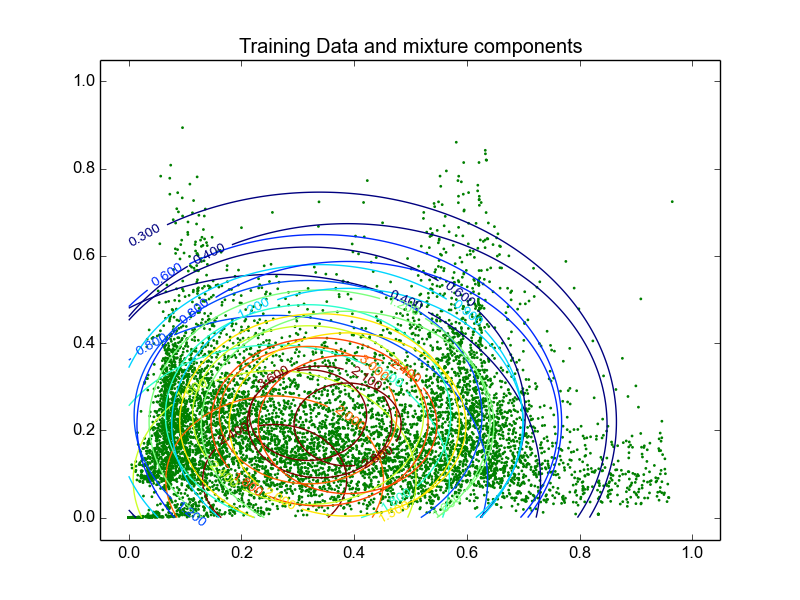
\includegraphics[width=.8\linewidth]{Figures/contours_diagstreet5.png}

  \label{fig:sfig1}
\end{figure}%
\end{minipage}
\begin{minipage}[b]{0.25\textwidth}
\begin{figure}[H]
  \centering
  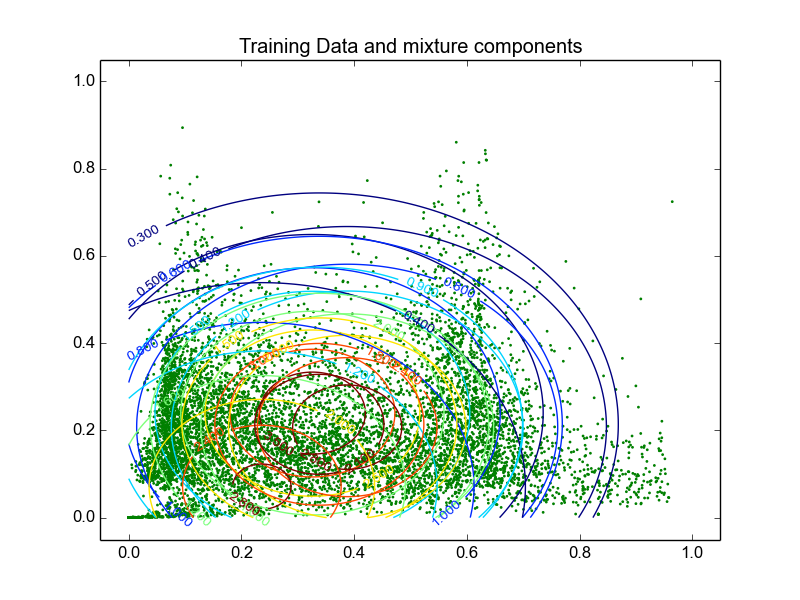
\includegraphics[width=.8\linewidth]{Figures/contours_diagstreet15.png}

  \label{fig:sfig1}
\end{figure}%
\end{minipage}
\begin{minipage}[b]{0.25\textwidth}
\begin{figure}[H]
  \centering
  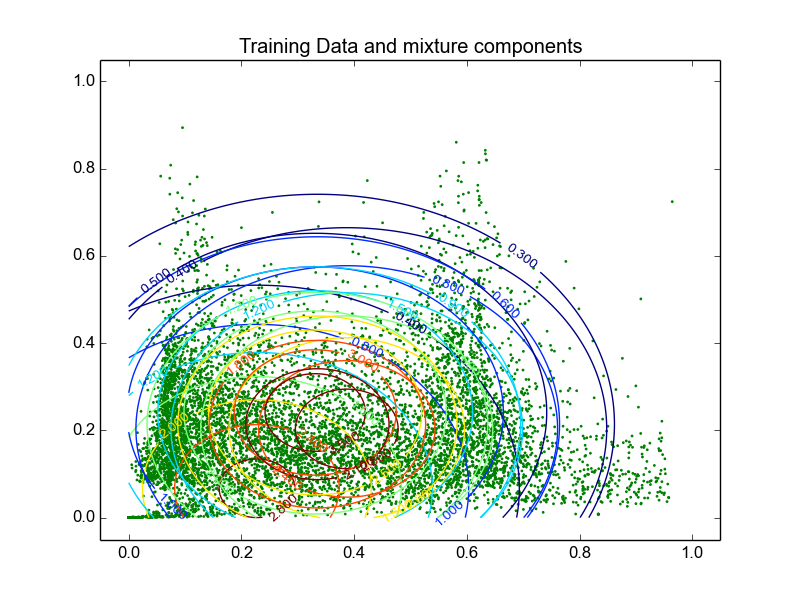
\includegraphics[width=.8\linewidth]{Figures/contours_diagstreet30.png}

  \label{fig:sfig1}
\end{figure}%
\end{minipage}
\subsection{Results}
\subsection{Log Likelihood}
\begin{minipage}[b]{0.5\textwidth}
\begin{figure}[H]
  \centering
  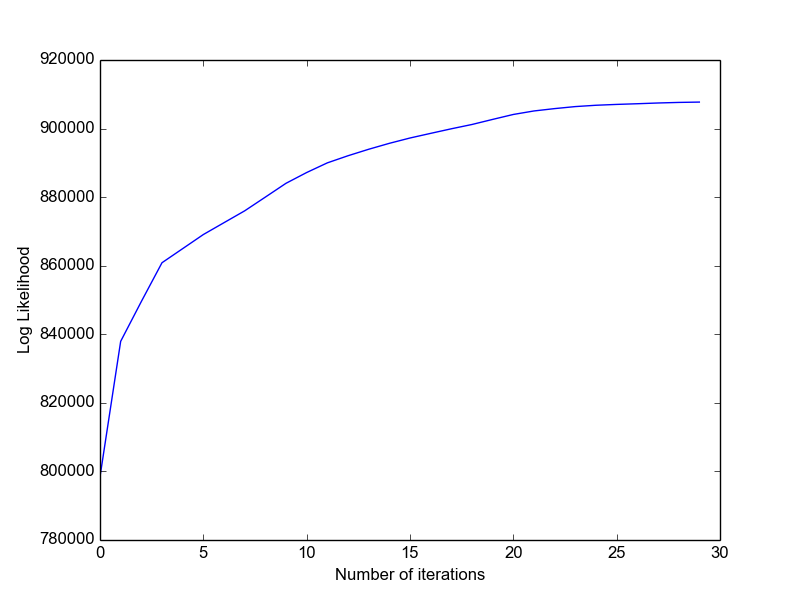
\includegraphics[width=.8\linewidth]{Figures/likelihood0.png}
  \caption{Confusion Matrix for full covariance}
  \label{fig:sfig1}
\end{figure}%
\end{minipage}
\begin{minipage}[b]{0.5\textwidth}
\begin{figure}[H]
  \centering
  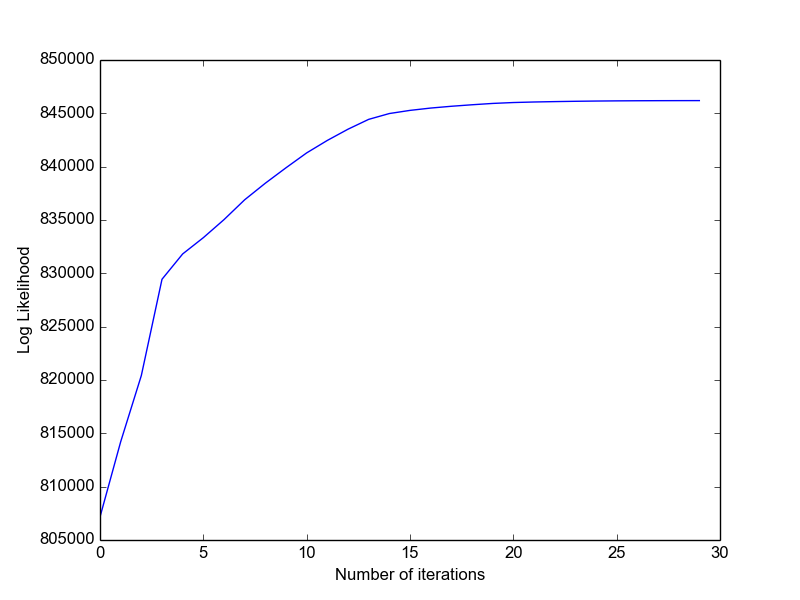
\includegraphics[width=.8\linewidth]{Figures/likelihood1.png}
\caption{Confusion Matrix for Diagonal Covariance}
  \label{fig:sfig1}
\end{figure}%
\end{minipage}
\begin{minipage}[b]{0.5\textwidth}
\begin{figure}[H]
  \centering
  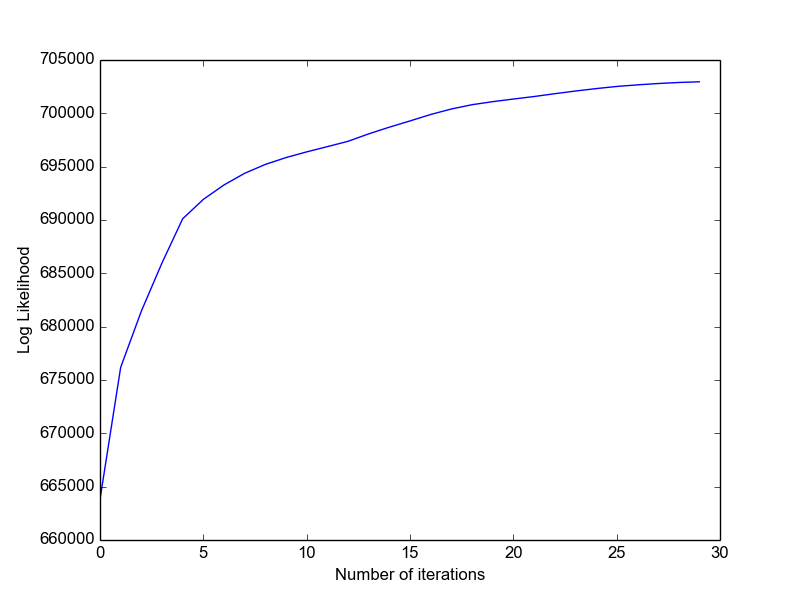
\includegraphics[width=.8\linewidth]{Figures/likelihood2.png}
\caption{Confusion Matrix for Diagonal Covariance}
  \label{fig:sfig1}
\end{figure}%
\end{minipage}

\subsection{Confusion Matrices}

\begin{minipage}[b]{0.5\textwidth}
\begin{figure}[H]
  \centering
  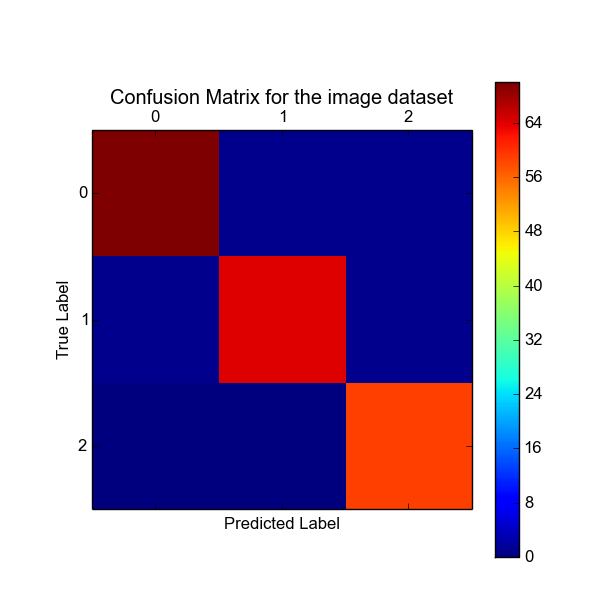
\includegraphics[width=.8\linewidth]{Figures/gmm_images_confusion.png}
  \caption{Confusion Matrix for full covariance}
  \label{fig:sfig1}
\end{figure}%
\end{minipage}
\begin{minipage}[b]{0.5\textwidth}
\begin{figure}[H]
  \centering
  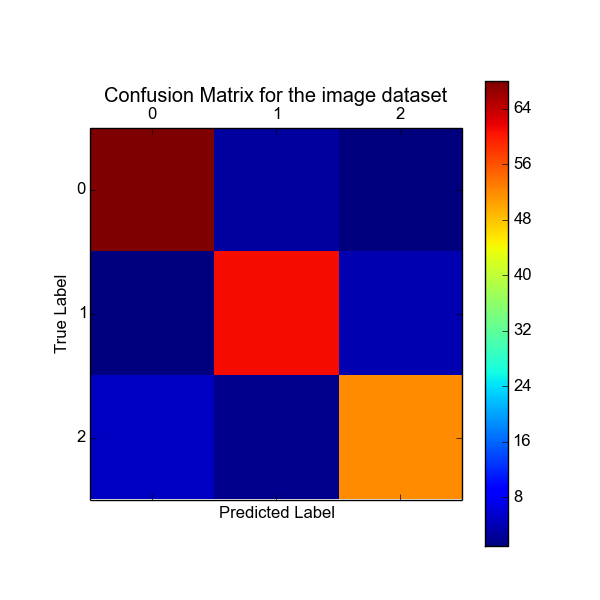
\includegraphics[width=.8\linewidth]{Figures/confusion_diag.png}
\caption{Confusion Matrix for Diagonal Covariance}
  \label{fig:sfig1}
\end{figure}%
\end{minipage}

\subsection{Precision and Recall}

\begin{minipage}[b]{0.5\textwidth}
\begin{figure}[H]
  \centering
  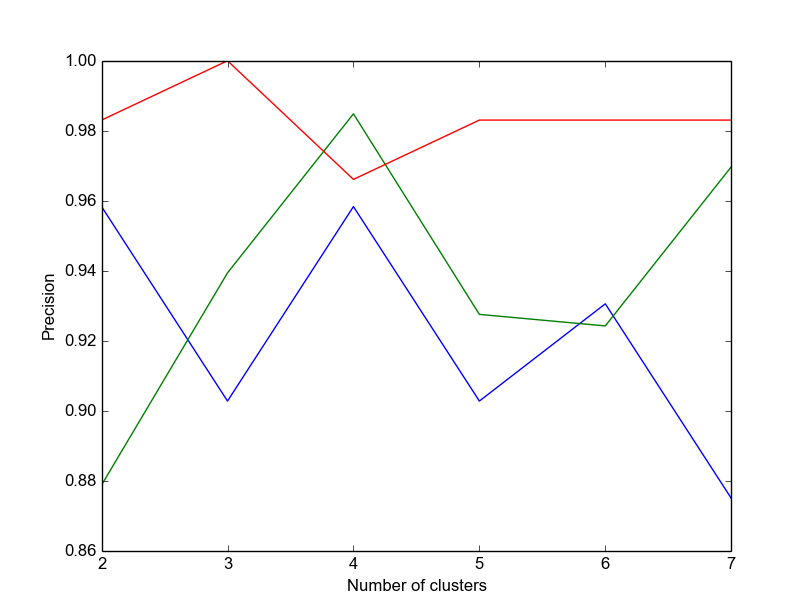
\includegraphics[width=.8\linewidth]{Figures/GMM_precisionvsk_BGR.png}
  \caption{Precision}
  \label{fig:sfig1}
\end{figure}%
\end{minipage}
\begin{minipage}[b]{0.5\textwidth}
\begin{figure}[H]
  \centering
  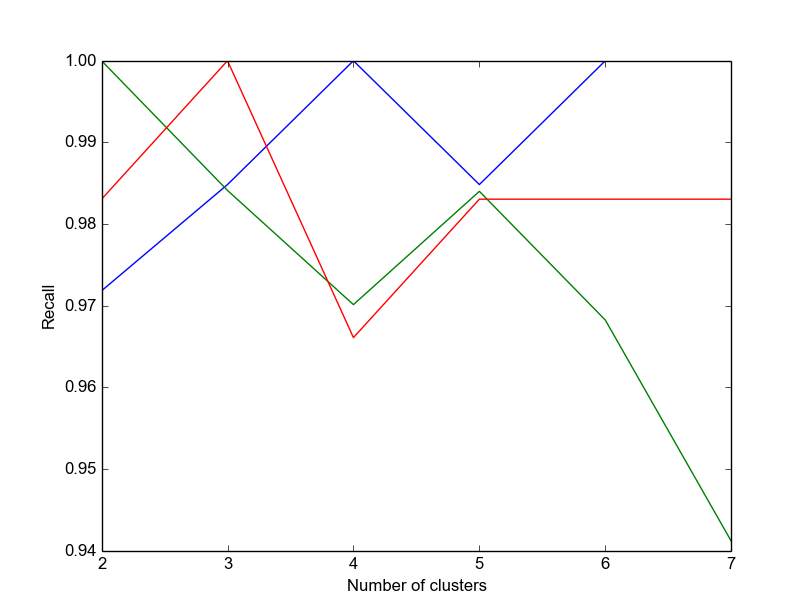
\includegraphics[width=.8\linewidth]{Figures/GMM_recallvsk_BGR.png}
\caption{Recall}
  \label{fig:sfig1}
\end{figure}%
\end{minipage}
\\

\section{Digit dataset}
Number of clusters per class: 2
\\Following figures show mixture components for iterations 0, 5, 15 and 20. 
\subsection{Eight}
\begin{minipage}[b]{0.25\textwidth}
\begin{figure}[H]
  \centering
  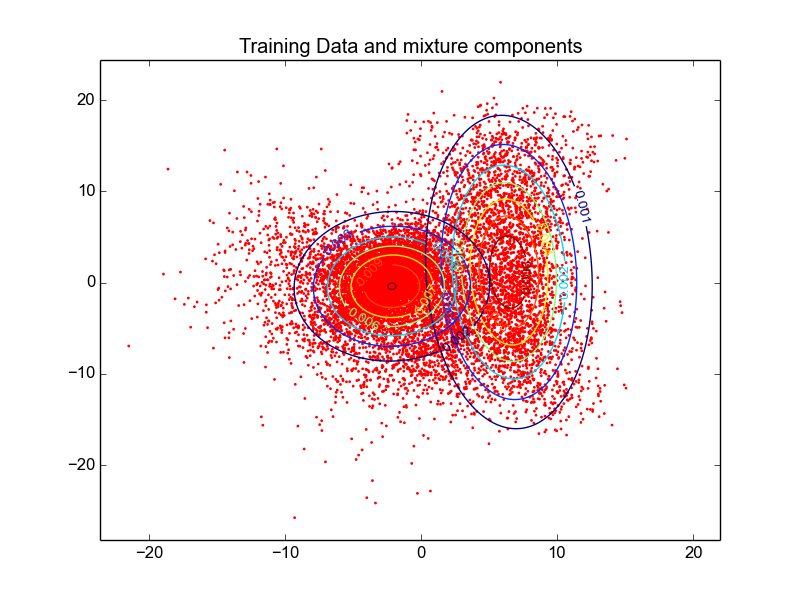
\includegraphics[width=.8\linewidth]{Figures/contours_digiteight0.png}
  \label{fig:sfig1}
\end{figure}%
\end{minipage}
\begin{minipage}[b]{0.25\textwidth}
\begin{figure}[H]
  \centering
  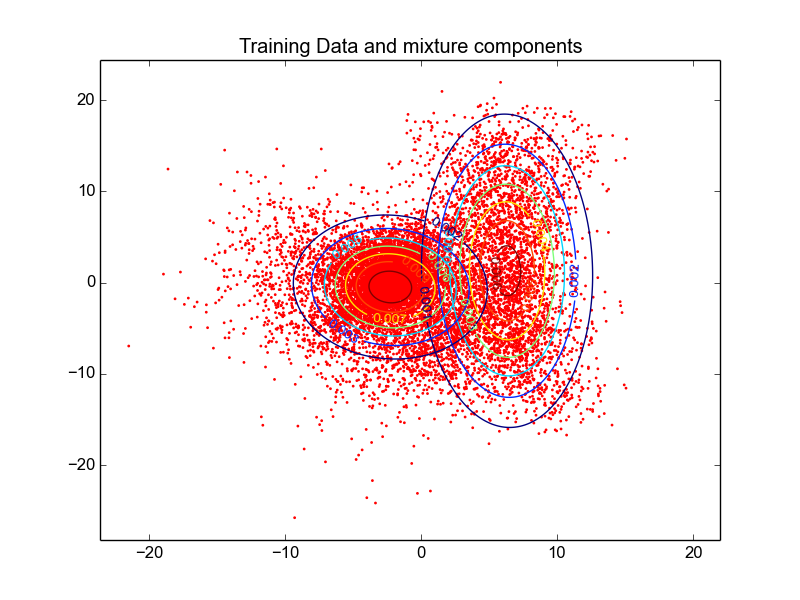
\includegraphics[width=.8\linewidth]{Figures/contours_digiteight5.png}

  \label{fig:sfig1}
\end{figure}%
\end{minipage}
\begin{minipage}[b]{0.25\textwidth}
\begin{figure}[H]
  \centering
  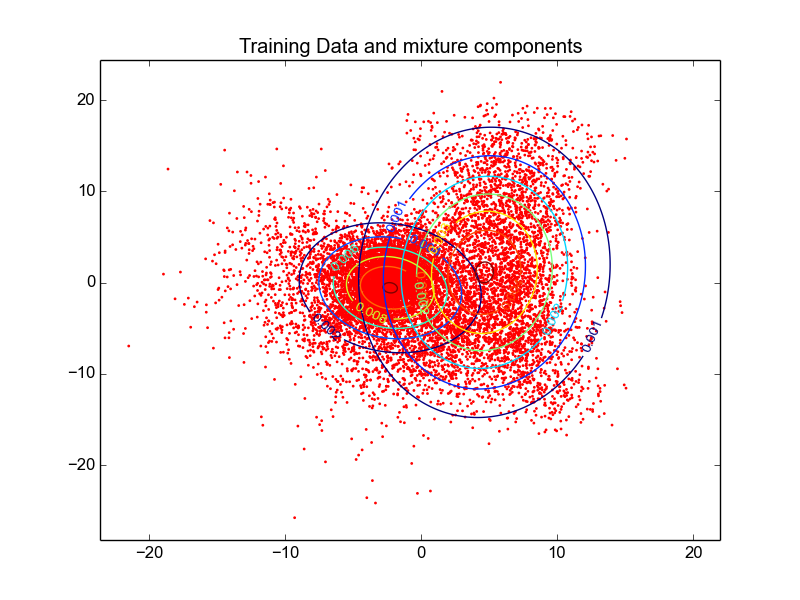
\includegraphics[width=.8\linewidth]{Figures/contours_digiteight15.png}

  \label{fig:sfig1}
\end{figure}%
\end{minipage}
\begin{minipage}[b]{0.25\textwidth}
\begin{figure}[H]
  \centering
  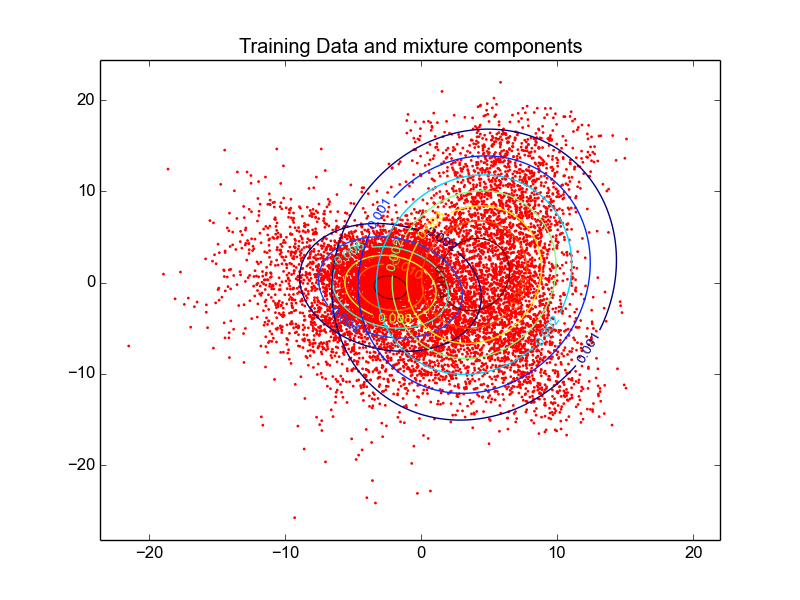
\includegraphics[width=.8\linewidth]{Figures/contours_digiteight20.png}
 \label{fig:sfig1}
\end{figure}%
\end{minipage}
\subsection{Seven}
Full Scatterplot: \\
\begin{minipage}[b]{0.25\textwidth}
\begin{figure}[H]
  \centering
  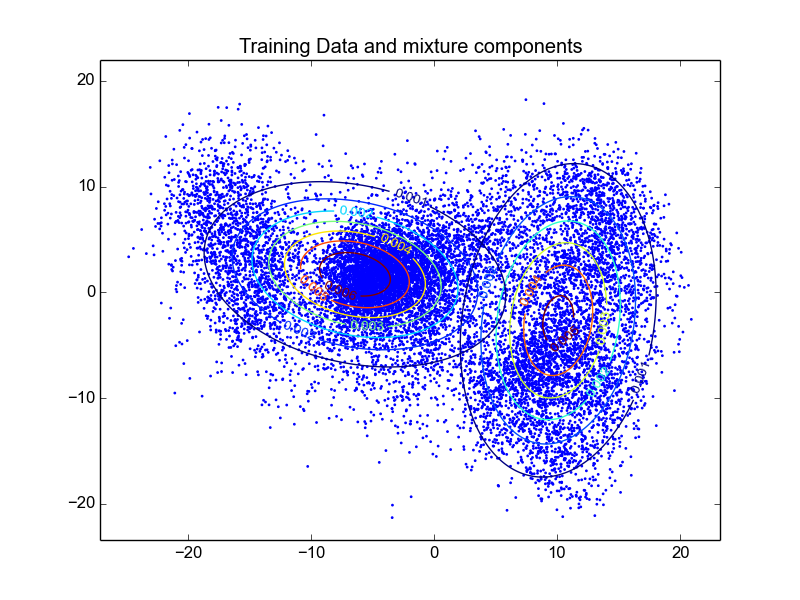
\includegraphics[width=.8\linewidth]{Figures/contours_digitseven0.png}
  \label{fig:sfig1}
\end{figure}%
\end{minipage}
\begin{minipage}[b]{0.25\textwidth}
\begin{figure}[H]
  \centering
  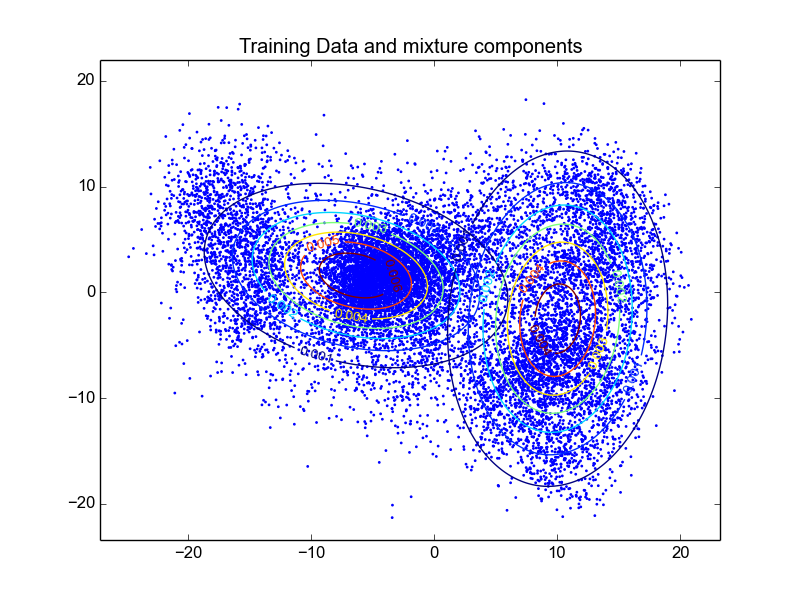
\includegraphics[width=.8\linewidth]{Figures/contours_digitseven5.png}

  \label{fig:sfig1}
\end{figure}%
\end{minipage}
\begin{minipage}[b]{0.25\textwidth}
\begin{figure}[H]
  \centering
  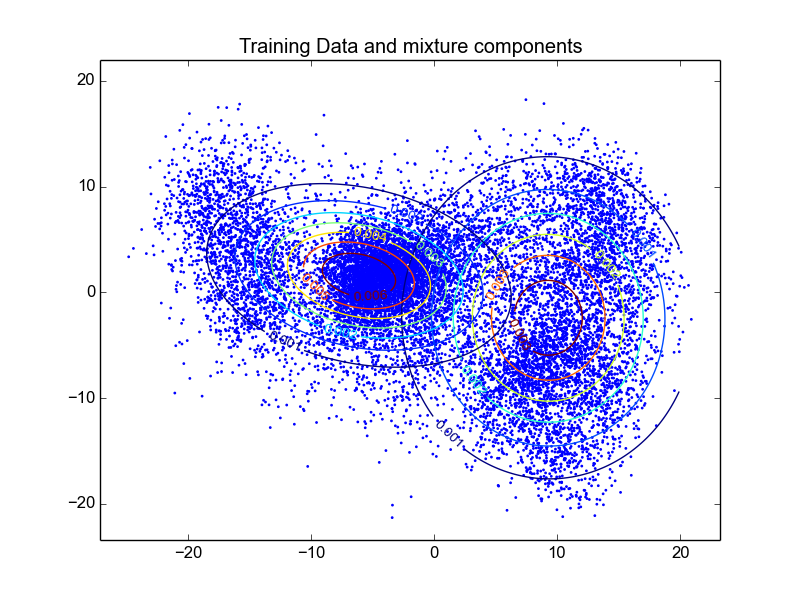
\includegraphics[width=.8\linewidth]{Figures/contours_digitseven15.png}

  \label{fig:sfig1}
\end{figure}%
\end{minipage}
\begin{minipage}[b]{0.25\textwidth}
\begin{figure}[H]
  \centering
  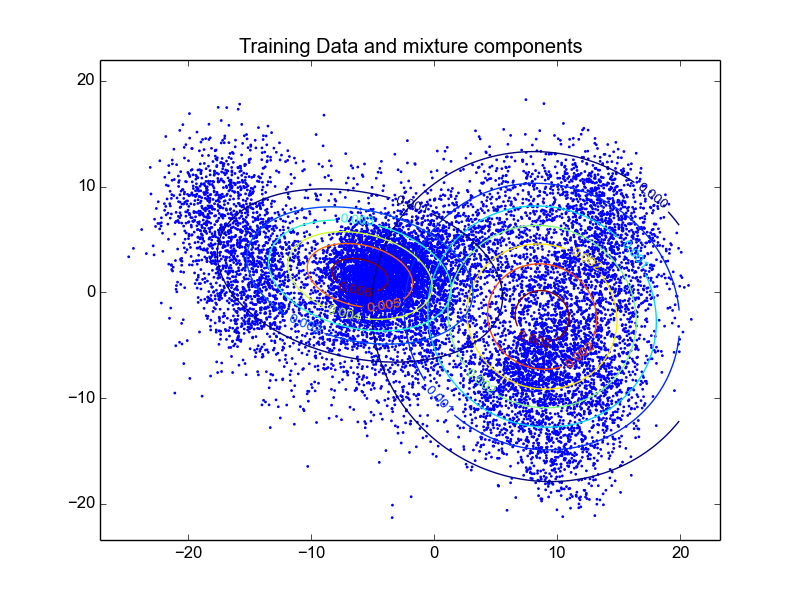
\includegraphics[width=.8\linewidth]{Figures/contours_digitseven20.png}

  \label{fig:sfig1}
\end{figure}%
\end{minipage}

\subsection{Six}
Full Scatterplot: \\
\begin{minipage}[b]{0.25\textwidth}
\begin{figure}[H]
  \centering
  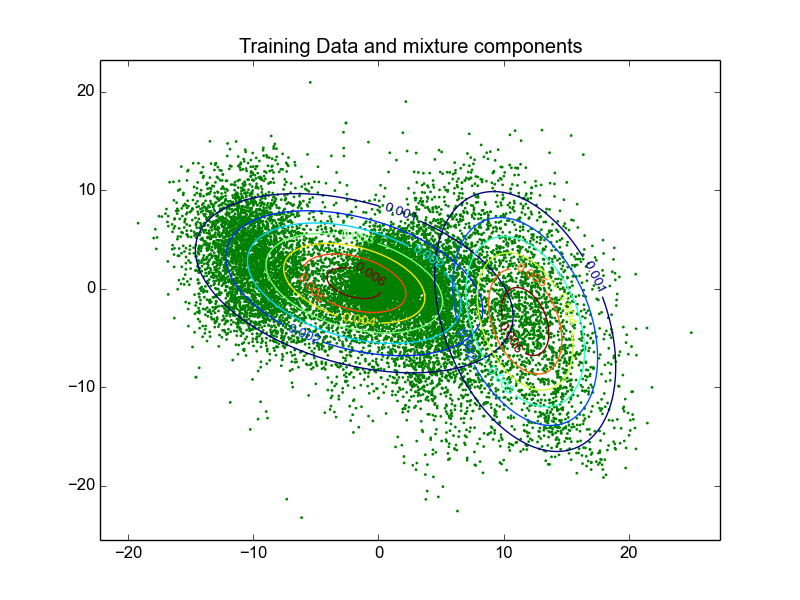
\includegraphics[width=.8\linewidth]{Figures/contours_digitsix0.png}
  \label{fig:sfig1}
\end{figure}%
\end{minipage}
\begin{minipage}[b]{0.25\textwidth}
\begin{figure}[H]
  \centering
  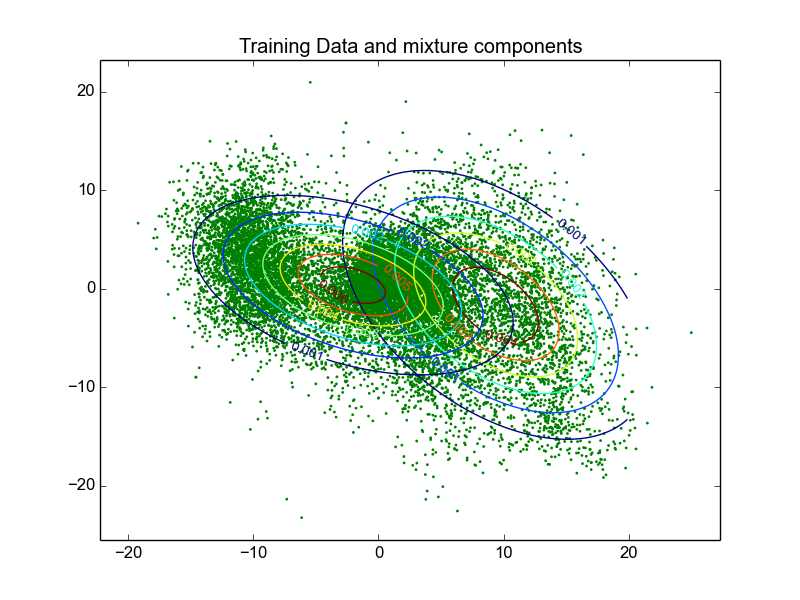
\includegraphics[width=.8\linewidth]{Figures/contours_digitsix5.png}

  \label{fig:sfig1}
\end{figure}%
\end{minipage}
\begin{minipage}[b]{0.25\textwidth}
\begin{figure}[H]
  \centering
  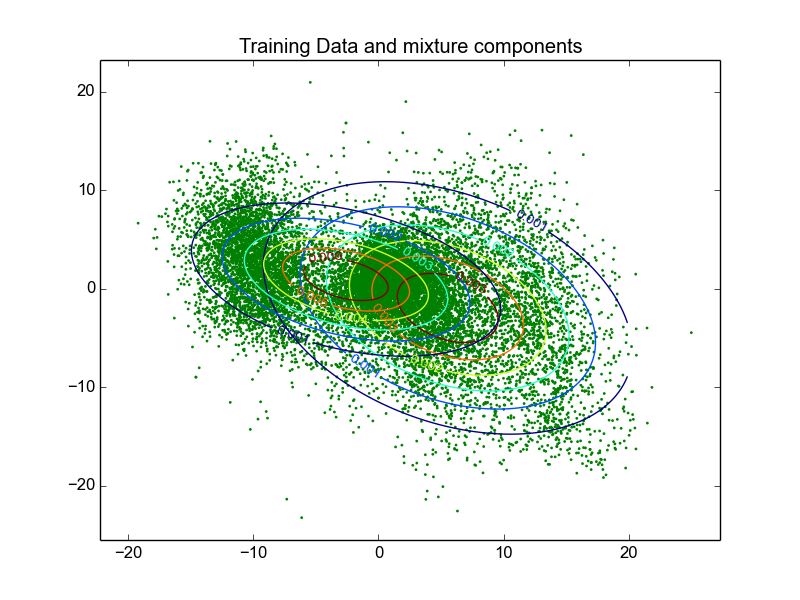
\includegraphics[width=.8\linewidth]{Figures/contours_digitsix15.png}

  \label{fig:sfig1}
\end{figure}%
\end{minipage}
\begin{minipage}[b]{0.25\textwidth}
\begin{figure}[H]
  \centering
  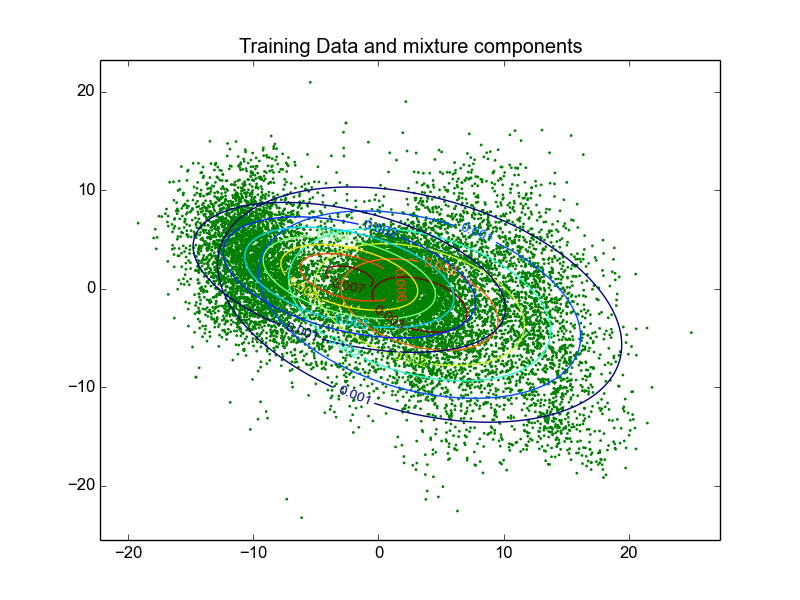
\includegraphics[width=.8\linewidth]{Figures/contours_digitsix20.png}

  \label{fig:sfig1}
\end{figure}%
\end{minipage}

\subsection{Three}
Full Scatterplot: \\
\begin{minipage}[b]{0.25\textwidth}
\begin{figure}[H]
  \centering
  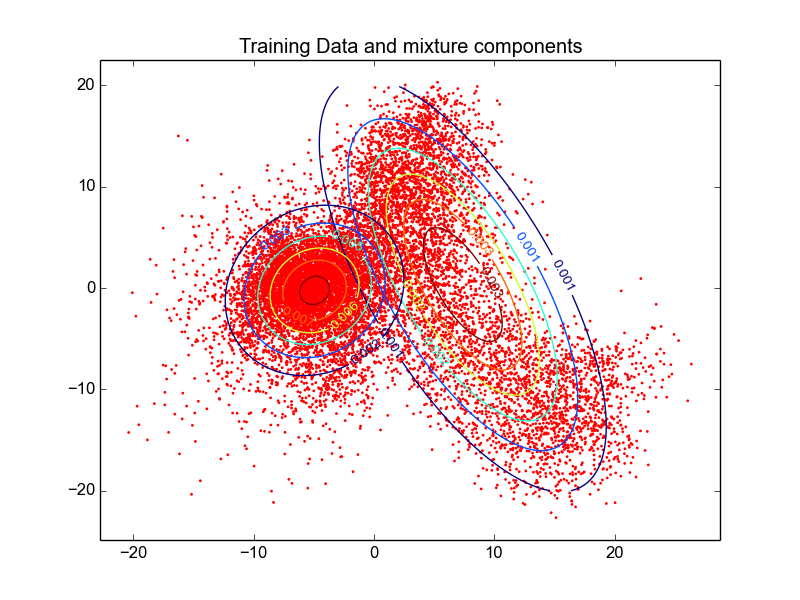
\includegraphics[width=.8\linewidth]{Figures/contours_digitthree0.png}
  \label{fig:sfig1}
\end{figure}%
\end{minipage}
\begin{minipage}[b]{0.25\textwidth}
\begin{figure}[H]
  \centering
  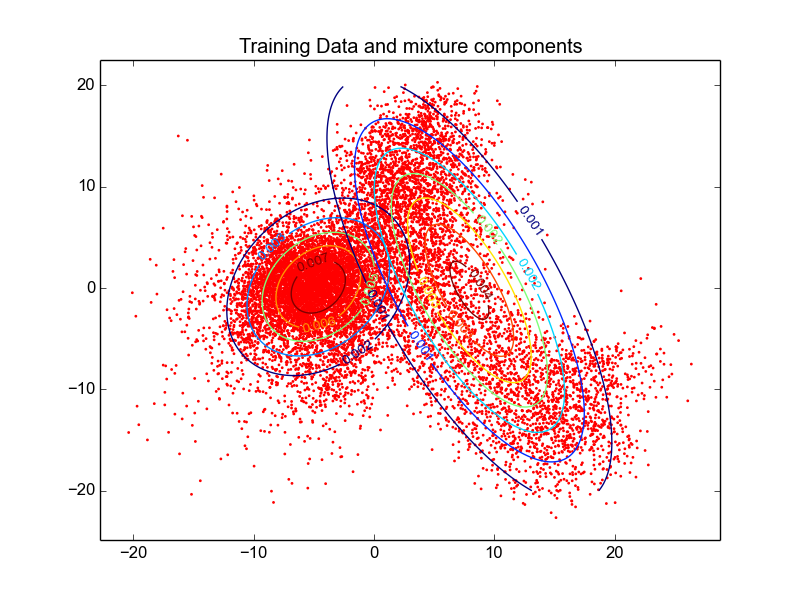
\includegraphics[width=.8\linewidth]{Figures/contours_digitthree5.png}

  \label{fig:sfig1}
\end{figure}%
\end{minipage}
\begin{minipage}[b]{0.25\textwidth}
\begin{figure}[H]
  \centering
  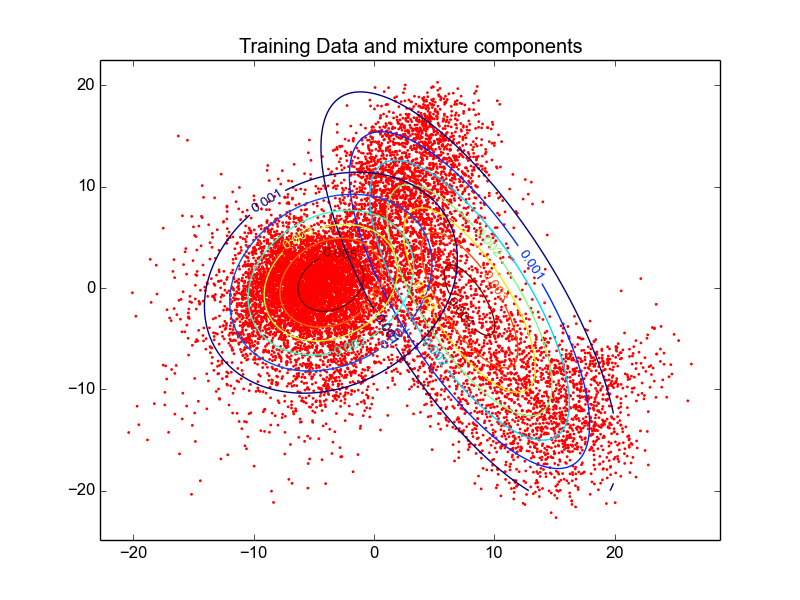
\includegraphics[width=.8\linewidth]{Figures/contours_digitthree15.png}

  \label{fig:sfig1}
\end{figure}%
\end{minipage}
\begin{minipage}[b]{0.25\textwidth}
\begin{figure}[H]
  \centering
  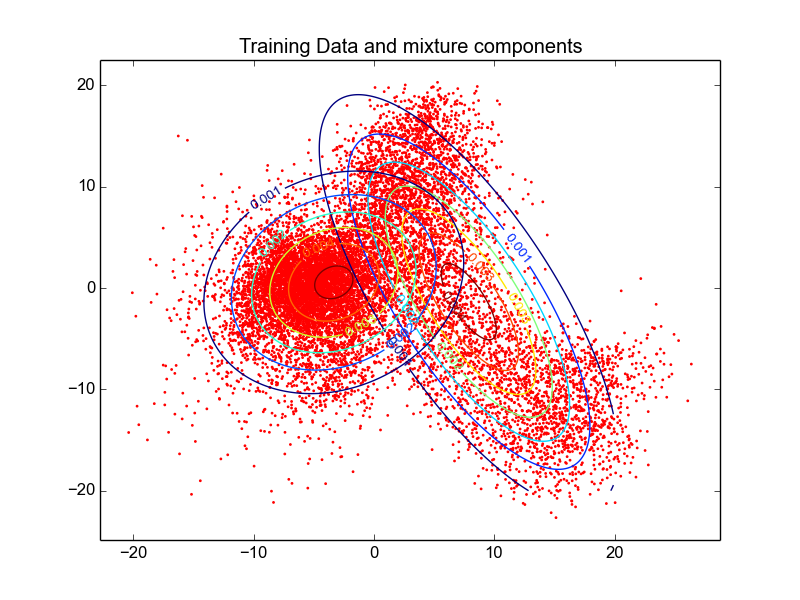
\includegraphics[width=.8\linewidth]{Figures/contours_digitthree20.png}

  \label{fig:sfig1}
\end{figure}%
\end{minipage}

\subsection{Two}
Full Scatterplot: \\
\begin{minipage}[b]{0.25\textwidth}
\begin{figure}[H]
  \centering
  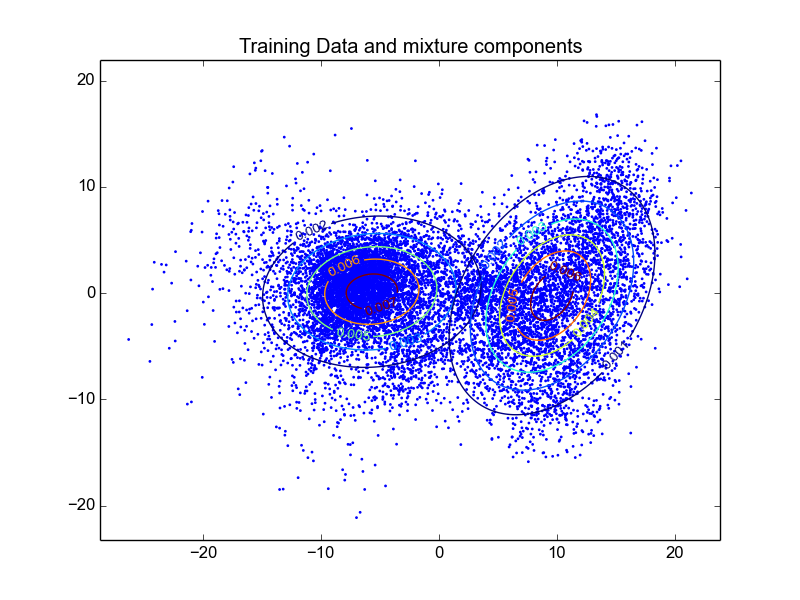
\includegraphics[width=.8\linewidth]{Figures/contours_digittwo0.png}
  \label{fig:sfig1}
\end{figure}%
\end{minipage}
\begin{minipage}[b]{0.25\textwidth}
\begin{figure}[H]
  \centering
  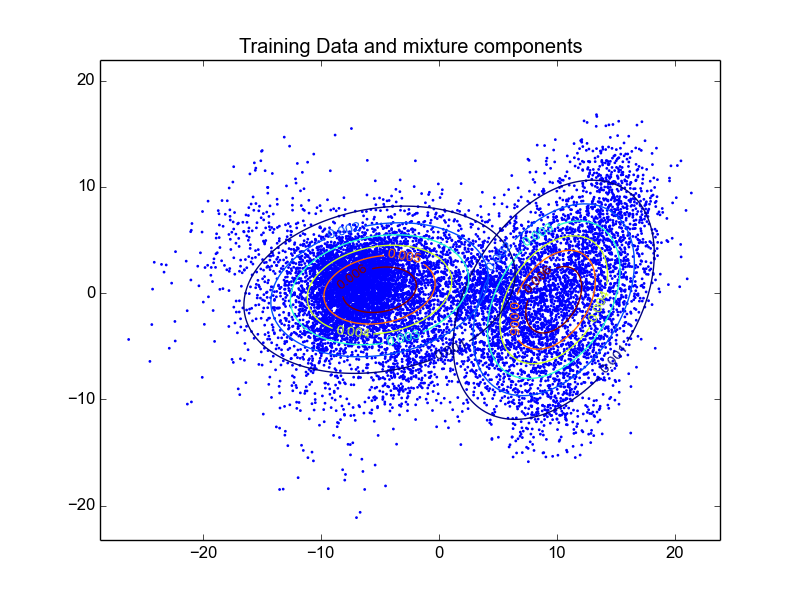
\includegraphics[width=.8\linewidth]{Figures/contours_digittwo5.png}

  \label{fig:sfig1}
\end{figure}%
\end{minipage}
\begin{minipage}[b]{0.25\textwidth}
\begin{figure}[H]
  \centering
  \includegraphics[width=.8\linewidth]{Figures/contours_digittwo15.png}

  \label{fig:sfig1}
\end{figure}%
\end{minipage}
\begin{minipage}[b]{0.25\textwidth}
\begin{figure}[H]
  \centering
  \includegraphics[width=.8\linewidth]{Figures/contours_digittwo20.png}

  \label{fig:sfig1}
\end{figure}%
\end{minipage}
\subsection{Results}

\subsection{Log Likelihood}
\begin{minipage}[b]{0.5\textwidth}
\begin{figure}[H]
  \centering
  \includegraphics[width=.8\linewidth]{Figures/likelihood_digits0.png}
  \caption{Confusion Matrix for full covariance}
  \label{fig:sfig1}
\end{figure}%
\end{minipage}
\begin{minipage}[b]{0.5\textwidth}
\begin{figure}[H]
  \centering
  \includegraphics[width=.8\linewidth]{Figures/likelihood_digits1.png}
\caption{Confusion Matrix for Diagonal Covariance}
  \label{fig:sfig1}
\end{figure}%
\end{minipage}
\begin{minipage}[b]{0.5\textwidth}
\begin{figure}[H]
  \centering
  \includegraphics[width=.8\linewidth]{Figures/likelihood_digits2.png}
\caption{Confusion Matrix for Diagonal Covariance}
  \label{fig:sfig1}
\end{figure}%
\end{minipage}
\begin{minipage}[b]{0.5\textwidth}
\begin{figure}[H]
  \centering
  \includegraphics[width=.8\linewidth]{Figures/likelihood_digits3.png}
\caption{Confusion Matrix for Diagonal Covariance}
  \label{fig:sfig1}
\end{figure}%
\end{minipage}
\begin{minipage}[b]{0.5\textwidth}
\begin{figure}[H]
  \centering
  \includegraphics[width=.8\linewidth]{Figures/likelihood_digits4.png}
\caption{Confusion Matrix for Diagonal Covariance}
  \label{fig:sfig1}
\end{figure}%
\end{minipage}

\subsection{Confusion Matrices}

\begin{minipage}[b]{0.5\textwidth}
\begin{figure}[H]
  \centering
  \includegraphics[width=.8\linewidth]{Figures/confusion_digit.png}
  \caption{Confusion Matrix for Digit}
  \label{fig:sfig1}
\end{figure}%
\end{minipage}

\subsection{Precision and Recall}

\begin{center}
\begin{tabular}{|c|c|}
\hline
\textbf{Precision} & \textbf{Recall} \\ \hline
1.0 & 1.0 \\ \hline
1.0 & 1.0 \\ \hline
1.0 & 1.0 \\ \hline
1.0 & 1.0 \\ \hline
1.0 & 1.0 \\ \hline
\end{tabular}

\end{center}

\section{Handwriting dataset}
Number of clusters per class: 5
\\Following figures show mixture components for iterations 0, 5, 10 and 15. 
\subsection{a}
\begin{minipage}[b]{0.25\textwidth}
\begin{figure}[H]
  \centering
  \includegraphics[width=.8\linewidth]{{Figures/contours_a.test0}.png}
  \label{fig:sfig1}
\end{figure}%
\end{minipage}
\begin{minipage}[b]{0.25\textwidth}
\begin{figure}[H]
  \centering
  \includegraphics[width=.8\linewidth]{{Figures/contours_a.test5}.png}

  \label{fig:sfig1}
\end{figure}%
\end{minipage}
\begin{minipage}[b]{0.25\textwidth}
\begin{figure}[H]
  \centering
  \includegraphics[width=.8\linewidth]{{Figures/contours_a.test10}.png}

  \label{fig:sfig1}
\end{figure}%
\end{minipage}
\begin{minipage}[b]{0.25\textwidth}
\begin{figure}[H]
  \centering
  \includegraphics[width=.8\linewidth]{{Figures/contours_a.test15}.png}
 \label{fig:sfig1}
\end{figure}%
\end{minipage}
\subsection{ai}
Full Scatterplot: \\
\begin{minipage}[b]{0.25\textwidth}
\begin{figure}[H]
  \centering
  \includegraphics[width=.8\linewidth]{{Figures/contours_ai.test0}.png}
  \label{fig:sfig1}
\end{figure}%
\end{minipage}
\begin{minipage}[b]{0.25\textwidth}
\begin{figure}[H]
  \centering
  \includegraphics[width=.8\linewidth]{{Figures/contours_ai.test5}.png}

  \label{fig:sfig1}
\end{figure}%
\end{minipage}
\begin{minipage}[b]{0.25\textwidth}
\begin{figure}[H]
  \centering
  \includegraphics[width=.8\linewidth]{{Figures/contours_ai.test10}.png}

  \label{fig:sfig1}
\end{figure}%
\end{minipage}
\begin{minipage}[b]{0.25\textwidth}
\begin{figure}[H]
  \centering
  \includegraphics[width=.8\linewidth]{{Figures/contours_ai.test15}.png}

  \label{fig:sfig1}
\end{figure}%
\end{minipage}

\subsection{bA}
Full Scatterplot: \\
\begin{minipage}[b]{0.25\textwidth}
\begin{figure}[H]
  \centering
  \includegraphics[width=.8\linewidth]{{Figures/contours_bA.test0}.png}
  \label{fig:sfig1}
\end{figure}%
\end{minipage}
\begin{minipage}[b]{0.25\textwidth}
\begin{figure}[H]
  \centering
  \includegraphics[width=.8\linewidth]{{Figures/contours_bA.test5}.png}

  \label{fig:sfig1}
\end{figure}%
\end{minipage}
\begin{minipage}[b]{0.25\textwidth}
\begin{figure}[H]
  \centering
  \includegraphics[width=.8\linewidth]{{Figures/contours_bA.test10}.png}

  \label{fig:sfig1}
\end{figure}%
\end{minipage}
\begin{minipage}[b]{0.25\textwidth}
\begin{figure}[H]
  \centering
  \includegraphics[width=.8\linewidth]{{Figures/contours_bA.test15}.png}

  \label{fig:sfig1}
\end{figure}%
\end{minipage}

\subsection{chA}
Full Scatterplot: \\
\begin{minipage}[b]{0.25\textwidth}
\begin{figure}[H]
  \centering
  \includegraphics[width=.8\linewidth]{{Figures/contours_chA.test0}.png}
  \label{fig:sfig1}
\end{figure}%
\end{minipage}
\begin{minipage}[b]{0.25\textwidth}
\begin{figure}[H]
  \centering
  \includegraphics[width=.8\linewidth]{{Figures/contours_chA.test5}.png}

  \label{fig:sfig1}
\end{figure}%
\end{minipage}
\begin{minipage}[b]{0.25\textwidth}
\begin{figure}[H]
  \centering
  \includegraphics[width=.8\linewidth]{{Figures/contours_chA.test10}.png}

  \label{fig:sfig1}
\end{figure}%
\end{minipage}
\begin{minipage}[b]{0.25\textwidth}
\begin{figure}[H]
  \centering
  \includegraphics[width=.8\linewidth]{{Figures/contours_chA.test15}.png}

  \label{fig:sfig1}
\end{figure}%
\end{minipage}

\subsection{dA}
Full Scatterplot: \\
\begin{minipage}[b]{0.25\textwidth}
\begin{figure}[H]
  \centering
  \includegraphics[width=.8\linewidth]{{Figures/contours_dA.test0}.png}
  \label{fig:sfig1}
\end{figure}%
\end{minipage}
\begin{minipage}[b]{0.25\textwidth}
\begin{figure}[H]
  \centering
  \includegraphics[width=.8\linewidth]{{Figures/contours_dA.test5}.png}

  \label{fig:sfig1}
\end{figure}%
\end{minipage}
\begin{minipage}[b]{0.25\textwidth}
\begin{figure}[H]
  \centering
  \includegraphics[width=.8\linewidth]{{Figures/contours_dA.test10}.png}

  \label{fig:sfig1}
\end{figure}%
\end{minipage}
\begin{minipage}[b]{0.25\textwidth}
\begin{figure}[H]
  \centering
  \includegraphics[width=.8\linewidth]{{Figures/contours_dA.test15}.png}

  \label{fig:sfig1}
\end{figure}%
\end{minipage}


\subsection{lA}
Full Scatterplot: \\
\begin{minipage}[b]{0.25\textwidth}
\begin{figure}[H]
  \centering
  \includegraphics[width=.8\linewidth]{{Figures/contours_lA.test0}.png}
  \label{fig:sfig1}
\end{figure}%
\end{minipage}
\begin{minipage}[b]{0.25\textwidth}
\begin{figure}[H]
  \centering
  \includegraphics[width=.8\linewidth]{{Figures/contours_lA.test5}.png}

  \label{fig:sfig1}
\end{figure}%
\end{minipage}
\begin{minipage}[b]{0.25\textwidth}
\begin{figure}[H]
  \centering
  \includegraphics[width=.8\linewidth]{{Figures/contours_lA.test10}.png}

  \label{fig:sfig1}
\end{figure}%
\end{minipage}
\begin{minipage}[b]{0.25\textwidth}
\begin{figure}[H]
  \centering
  \includegraphics[width=.8\linewidth]{{Figures/contours_lA.test15}.png}

  \label{fig:sfig1}
\end{figure}%
\end{minipage}


\subsection{LA}
Full Scatterplot: \\
\begin{minipage}[b]{0.25\textwidth}
\begin{figure}[H]
  \centering
  \includegraphics[width=.8\linewidth]{{Figures/contours_LA.test0}.png}
  \label{fig:sfig1}
\end{figure}%
\end{minipage}
\begin{minipage}[b]{0.25\textwidth}
\begin{figure}[H]
  \centering
  \includegraphics[width=.8\linewidth]{{Figures/contours_LA.test5}.png}

  \label{fig:sfig1}
\end{figure}%
\end{minipage}
\begin{minipage}[b]{0.25\textwidth}
\begin{figure}[H]
  \centering
  \includegraphics[width=.8\linewidth]{{Figures/contours_LA.test10}.png}

  \label{fig:sfig1}
\end{figure}%
\end{minipage}
\begin{minipage}[b]{0.25\textwidth}
\begin{figure}[H]
  \centering
  \includegraphics[width=.8\linewidth]{{Figures/contours_LA.test15}.png}

  \label{fig:sfig1}
\end{figure}%
\end{minipage}


\subsection{tA}
Full Scatterplot: \\
\begin{minipage}[b]{0.25\textwidth}
\begin{figure}[H]
  \centering
  \includegraphics[width=.8\linewidth]{{Figures/contours_tA.test0}.png}
  \label{fig:sfig1}
\end{figure}%
\end{minipage}
\begin{minipage}[b]{0.25\textwidth}
\begin{figure}[H]
  \centering
  \includegraphics[width=.8\linewidth]{{Figures/contours_tA.test5}.png}

  \label{fig:sfig1}
\end{figure}%
\end{minipage}
\begin{minipage}[b]{0.25\textwidth}
\begin{figure}[H]
  \centering
  \includegraphics[width=.8\linewidth]{{Figures/contours_tA.test10}.png}

  \label{fig:sfig1}
\end{figure}%
\end{minipage}
\begin{minipage}[b]{0.25\textwidth}
\begin{figure}[H]
  \centering
  \includegraphics[width=.8\linewidth]{{Figures/contours_tA.test15}.png}

  \label{fig:sfig1}
\end{figure}%
\end{minipage}


\subsection{Results}

\subsection{Log Likelihood}
\begin{minipage}[b]{0.5\textwidth}
\begin{figure}[H]
  \centering
  \includegraphics[width=.8\linewidth]{Figures/likelihood_HW0.png}
  \caption{Confusion Matrix for full covariance}
  \label{fig:sfig1}
\end{figure}%
\end{minipage}
\begin{minipage}[b]{0.5\textwidth}
\begin{figure}[H]
  \centering
  \includegraphics[width=.8\linewidth]{Figures/likelihood_HW1.png}
\caption{Confusion Matrix for Diagonal Covariance}
  \label{fig:sfig1}
\end{figure}%
\end{minipage}
\begin{minipage}[b]{0.5\textwidth}
\begin{figure}[H]
  \centering
  \includegraphics[width=.8\linewidth]{Figures/likelihood_HW2.png}
\caption{Confusion Matrix for Diagonal Covariance}
  \label{fig:sfig1}
\end{figure}%
\end{minipage}
\begin{minipage}[b]{0.5\textwidth}
\begin{figure}[H]
  \centering
  \includegraphics[width=.8\linewidth]{Figures/likelihood_HW3.png}
\caption{Confusion Matrix for Diagonal Covariance}
  \label{fig:sfig1}
\end{figure}%
\end{minipage}

\begin{minipage}[b]{0.5\textwidth}
\begin{figure}[H]
  \centering
  \includegraphics[width=.8\linewidth]{Figures/likelihood_HW4.png}
\caption{Confusion Matrix for Diagonal Covariance}
  \label{fig:sfig1}
\end{figure}%
\end{minipage}
\begin{minipage}[b]{0.5\textwidth}
\begin{figure}[H]
  \centering
  \includegraphics[width=.8\linewidth]{Figures/likelihood_HW5.png}
\caption{Confusion Matrix for Diagonal Covariance}
  \label{fig:sfig1}
\end{figure}%
\end{minipage}

\begin{minipage}[b]{0.5\textwidth}
\begin{figure}[H]
  \centering
  \includegraphics[width=.8\linewidth]{Figures/likelihood_HW6.png}
\caption{Confusion Matrix for Diagonal Covariance}
  \label{fig:sfig1}
\end{figure}%
\end{minipage}

\begin{minipage}[b]{0.5\textwidth}
\begin{figure}[H]
  \centering
  \includegraphics[width=.8\linewidth]{Figures/likelihood_HW7.png}
\caption{Confusion Matrix for Diagonal Covariance}
  \label{fig:sfig1}
\end{figure}%
\end{minipage}

\subsection{Confusion Matrices}

\begin{minipage}[b]{0.5\textwidth}
\begin{figure}[H]
  \centering
  \includegraphics[width=.8\linewidth]{Figures/confusion_HW.png}
  \caption{Confusion Matrix for Digit}
  \label{fig:sfig1}
\end{figure}%
\end{minipage}

\subsection{Precision and Recall}

\begin{center}
\begin{tabular}{|c|c|}
\hline
\textbf{Precision} & \textbf{Recall} \\ \hline
0.5280 & 0.3548 \\ \hline
0.1 & 0.6666 \\ \hline
0.0588 & 1.0 \\ \hline
0.25 & 0.625 \\ \hline
0.3684 & 0.3043 \\ \hline
0.0 & 0.0 \\ \hline
0.5555 & 0.1851 \\ \hline
0.4210 & 0.2666 \\ \hline
\end{tabular}

\end{center}

\section{Spiral dataset}
Number of clusters per class: 10,15
\\Following figures show mixture components
\subsection{Mixture Components}
\begin{minipage}[b]{0.25\textwidth}
\begin{figure}[H]
  \centering
  \includegraphics[width=.8\linewidth]{Figures/contours_spiral05.png}
  \label{fig:sfig1}
\end{figure}%
\end{minipage}
\begin{minipage}[b]{0.25\textwidth}
\begin{figure}[H]
  \centering
  \includegraphics[width=.8\linewidth]{Figures/contours_spiral15.png}

  \label{fig:sfig1}
\end{figure}%
\end{minipage}
\subsection{Results}

\subsection{Log Likelihood}
\begin{minipage}[b]{0.5\textwidth}
\begin{figure}[H]
  \centering
  \includegraphics[width=.8\linewidth]{Figures/likelihood_spiral0.png}
  \caption{Confusion Matrix for full covariance}
  \label{fig:sfig1}
\end{figure}%
\end{minipage}
\begin{minipage}[b]{0.5\textwidth}
\begin{figure}[H]
  \centering
  \includegraphics[width=.8\linewidth]{Figures/likelihood_spiral1.png}
\caption{Confusion Matrix for Diagonal Covariance}
  \label{fig:sfig1}
\end{figure}%
\end{minipage}

\subsection{Precision and Recall}

\begin{center}
\begin{tabular}{|c|c|}
\hline
\textbf{Precision} & \textbf{Recall} \\ \hline
1.0 & 1.0 \\ \hline
1.0 & 1.0 \\ \hline
\end{tabular}

\end{center}


\section{Hidden Markov Models}
\subsection{Solution Methodology}
The feature vectors were first quantized using a K-means clustering with number of clusters varying from 8 to 16. From this, a new quantized feature set was developed which was used as input to the HMM. This was then tested with the test set, from the given data which was clustered with the given means, to form the  quantized test data. We train a HMM for each class, and the class with maximum emission probability is assigned to the test data. The results are as follows
\subsection{Image Dataset}
\begin{figure}[H]
  \centering
  \includegraphics[width=.8\linewidth]{confusion_image_2.png}
\caption{Confusion matrix for HMM}
  \label{fig:sfig1}
\end{figure}%
\begin{center}
\begin{tabular}{|c|c|}
\hline
\textbf{Precision} & \textbf{Recall} \\ \hline
0.487179487179 & 0.95 \\ \hline
0.68115942029 & 0.783333333333 \\ \hline
0.941860465116 & 0.609022556391 \\ \hline
\end{tabular}

\end{center}
\subsection{Digits Dataset}
\begin{figure}[H]
  \centering
  \includegraphics[width=.8\linewidth]{Figures/confusion_digit_HMM.png}
\caption{Confusion matrix for HMM Digits}
  \label{fig:sfig1}
\end{figure}%
\begin{center}
\begin{tabular}{|c|c|c|c|c|c|}
\hline
\textbf{Precision} & 0.75 & 0.84 & 1.0 & 1.0 & 1.0 \\ \hline
\textbf{Recall} & 1.0 & 1.0 & 0.86 & 0.86 & 0.91 \\ \hline
\end{tabular}
\end{center}
\section{Conclusion}
From the exercise, it is clear that GMMs and HMMs are good at different classification tasks. HMMs outperform GMM for sequential data, while GMMs are far superior when it comes to data with spatial features. HMMs work well with temporal features.
\end{document}